\documentclass[11pt]{article}
\usepackage[preprint]{acl}
\usepackage{times}
\usepackage{latexsym}
\usepackage[T1]{fontenc}
\usepackage[utf8]{inputenc}
\usepackage{microtype}
\usepackage{lmodern}
\renewcommand{\ttdefault}{lmtt}
\renewcommand{\rmdefault}{ptm}
\renewcommand{\sfdefault}{phv}
\usepackage{graphicx}
\usepackage{booktabs}
\usepackage{adjustbox}
\usepackage{tabularx}
\usepackage{array}
\usepackage{enumitem}
\usepackage{newunicodechar}
\usepackage{morefloats}
\usepackage[section]{placeins}
\extrafloats{200}
\renewcommand{\topfraction}{0.95}
\renewcommand{\dbltopfraction}{0.95}
\renewcommand{\textfraction}{0.05}
\renewcommand{\floatpagefraction}{0.6}
\renewcommand{\dblfloatpagefraction}{0.6}
\setcounter{topnumber}{4}
\setcounter{dbltopnumber}{4}
\usepackage{tikz}
\usetikzlibrary{positioning,arrows.meta,calc}

\newunicodechar{−}{\ensuremath{-}}
\newunicodechar{×}{\ensuremath{\times}}
\newunicodechar{÷}{\ensuremath{\div}}
\newunicodechar{→}{\ensuremath{\rightarrow}}
\newunicodechar{≥}{\ensuremath{\geq}}
\newunicodechar{≤}{\ensuremath{\leq}}
\newunicodechar{≈}{\ensuremath{\approx}}
\newunicodechar{…}{\ldots}
\newunicodechar{·}{\ensuremath{\cdot}}
\newunicodechar{‑}{-}

\providecommand{\tightlist}{\setlength{\itemsep}{0pt}\setlength{\parskip}{0pt}}
\setlist{nosep,leftmargin=*}
\emergencystretch=3em
\hbadness=10000
\hfuzz=20pt
\setcounter{secnumdepth}{3}

\title{Intent-Gated Data Transformation Agent: Final Report}
\author{Team SSSS \\ LMA Group Project 2026}

\begin{document}
\maketitle
\begin{abstract}
Large language models (LLMs) are increasingly used to write
data-transformation code from natural-language requests. Such code often
runs without error but silently does the wrong thing: it removes valid
rows, changes columns the user did not mention, or deduplicates on the
wrong key. Conventional data-quality checks cannot reliably catch these
errors, because they do not know what the user asked for.

We propose an \textbf{intent-gated} pipeline. A parser turns each
request into an \textbf{intent contract}, a short list of checkable
statements in two halves: what the transformation \emph{must change} and
what it \emph{must preserve}. After the generated code runs in a
sandbox, a deterministic verifier compares the data before and after
against the contract. A bounded, tool-using repair agent then tries to
fix code that fails.

We ask two questions:

\begin{itemize}
\tightlist
\item
  Do intent contracts detect silent errors better than conventional
  checks?
\item
  Does an agent that combines an intent parser with a repair loop
  increase the accuracy of the transformations it delivers?
\end{itemize}

To answer them, we built a benchmark of 120 tasks on four public
datasets, each with reference code and a gold contract, and a frozen
pool of 803 LLM-written candidate programs labelled correct or wrong.

\textbf{Detection results (Stage 1, test split):}

\begin{itemize}
\tightlist
\item
  With gold contracts, the verifier catches 94.4\% of silently wrong
  programs with no false rejections. Conventional checks catch 45.5\%
  and wrongly reject 13.9\% of correct programs.
\item
  A QLoRA fine-tuned Qwen2.5-1.5B parser writes better contracts than a
  prompted Qwen2.5-7B model: 2\% invalid contracts vs 13\%, and 16.5\%
  false rejection vs 25.4\%.
\item
  Two later 1.5B parsers, one given request-relevant facts (selective
  facts) and one that can query the data with read-only tools (tool
  use), reach recall 0.944 / 0.930 and false rejection 0.120 / 0.139 on
  the same pool. Their false-rejection rate is lower than that of the
  first fine-tuned 1.5B parser (0.165), but the difference is within the
  confidence intervals (see Experiment 6b).
\end{itemize}

\textbf{Accuracy results (agent evaluation and Stage 2).}

\begin{itemize}
\tightlist
\item
  On the agent scenarios, the tool-using repair agent fixes 71\% of
  repairable programs, against about 61--62\% for simpler retry
  strategies.
\item
  End to end on the 100 test tasks, the repair loop raises the proposed
  system's correct outputs from 66 to 76.
\item
  The system accepts only 2 wrong outputs, against 20 for direct
  generation.
\item
  However, in this initial configuration it delivers about the same
  number of correct outputs as direct generation (76 vs 78), because
  imperfect contracts also reject correct code.
\item
  With gold contracts, the same agent solves 94 of 100 tasks.
\item
  In the final configuration, the selective-facts and tool-use parsers,
  a contract self-check, and a 3B repair agent with repair hints give 82
  and 80 correct outputs, with 2 and 1 wrong outputs accepted. Direct
  generation gives 78 correct outputs and 20 wrong accepted outputs. The
  gain in correct outputs is not statistically significant, while the
  reduction in wrong accepted outputs is large. With gold contracts this
  configuration solves 92 of 100 tasks.
\end{itemize}

Intent contracts therefore clearly improve error detection. They can
also raise accuracy, but only when the contracts are correct, which
makes contract quality the main bottleneck. No unsafe code was executed
in any run.

\end{abstract}

\section{Introduction}

\subsection{Motivation}

Data preparation, which includes filtering rows, removing duplicates,
handling missing values, converting types and deriving new columns, is a
large part of everyday data work. It is now common to ask an LLM to
write this code, for example as a pandas function, from a short request
such as "remove passengers younger than 18; unknown ages stay".

The main risk is not code that crashes; a crash is visible and easy to
handle. The risk is code that \textbf{runs successfully but does the
wrong thing}. In our candidate pool, even the stronger code generator
(Qwen2.5-3B) solved about one task in four wrongly with greedy decoding,
and about a third of the distinct programs that run are silently wrong.
Typical mistakes include:

\begin{itemize}
\tightlist
\item
  removing the right rows \emph{and some extra ones},
\item
  deduplicating on part of the requested key, or sorting first so that
  the wrong row is kept,
\item
  filling missing values in every column instead of one,
\item
  converting a column to the wrong type or category order,
\item
  leaving temporary helper columns in the output.
\end{itemize}

These errors are hard to notice because the output looks plausible.

Generic data-quality checks, such as row counts, null counts, type
checks and distribution shifts, are the usual safety net. They have one
basic limitation: they \textbf{do not know the user's intent}. A correct
filter that removes 20\% of the rows looks exactly like a faulty one
that removes 20\% of the rows by mistake. A request that should change a
column's distribution is indistinguishable from an unrequested change.

\subsection{Our approach}

We make the user's intent explicit and checkable. For each request, an
\textbf{intent parser} writes an \textbf{intent contract} in a small,
closed vocabulary of 11 predicate types (for example
\texttt{rows\_\allowbreak{}removed\_\allowbreak{}where},
\texttt{rows\_\allowbreak{}retained\_\allowbreak{}where},
\texttt{duplicate\_\allowbreak{}count} with a keep rule,
\texttt{column\_\allowbreak{}value\_\allowbreak{}relation},
\texttt{columns\_\allowbreak{}unchanged}). The contract has two halves:

\begin{itemize}
\tightlist
\item
  \textbf{\texttt{must\_\allowbreak{}change}} states what the request
  asks to change, e.g. "every row with Age \textless{} 18 is removed".
\item
  \textbf{\texttt{must\_\allowbreak{}preserve}} states what a reasonable
  user expects to stay the same even though they did not say so, e.g.
  "every row with Age ≥ 18 or unknown Age is kept, and no column
  changes".
\end{itemize}

After the generated code runs in a sandbox, a \textbf{deterministic
verifier} checks every predicate against the data before and after. No
LLM is used as a judge. If the check fails, a \textbf{repair agent}
reads a precise failure report, may inspect the data with read-only
tools, and proposes revised code, within a fixed budget. Unsafe code is
blocked by a static safety checker before it ever runs.

The project combines three capabilities:

\begin{itemize}
\tightlist
\item
  \textbf{Fine-tuning:} a small parser, trained with QLoRA, writes the
  contracts.
\item
  \textbf{Tool calling:} the repair agent uses a registry of
  data-inspection and execution tools.
\item
  \textbf{Agentic behaviour:} the agent decides between repairing,
  inspecting and escalating to a human, using a memory of its earlier
  attempts.
\end{itemize}

\subsection{Research question and hypotheses}

\textbf{Research question.} Does an intent contract that specifies what
must change and what must be preserved improve the detection of silent
semantic errors in LLM-generated data transformations, and does an agent
that combines such contracts with an intent parser and a repair loop
increase the accuracy of data transformations?

The question has two parts, each tested in its own stage of the
evaluation:

\begin{table*}[!tp]
\centering\footnotesize\setlength{\tabcolsep}{3pt}\renewcommand{\arraystretch}{1.1}
\begin{tabularx}{\textwidth}{l>{\raggedright\arraybackslash}X>{\raggedright\arraybackslash}X>{\raggedright\arraybackslash}X}
\toprule
\textbf{Part} & \textbf{Question} & \textbf{Compared against} & \textbf{Evaluated in} \\
\midrule
RQ1: detection & Do intent contracts detect silent semantic errors better than conventional data-quality checks? & No verification; conventional checks & Stage 1: every system judges the same frozen pool of LLM-written programs \\
RQ2: accuracy & Does the full agent (intent parser + contract-checked generation + repair loop) deliver more correct transformations? & Direct generation; conventional checks + repair; prompted-parser contracts + repair & Stage 2: the full pipeline runs end to end on the 100 test tasks \\
\bottomrule
\end{tabularx}
\end{table*}

\textbf{Hypotheses.}

\begin{itemize}
\tightlist
\item
  \textbf{H1 (detection):} intent-based verification will accept fewer
  incorrect transformations than conventional checks while keeping the
  false-rejection rate low.
\item
  \textbf{H2 (accuracy):} the intent-gated agent with repair will
  deliver more correct accepted outputs than direct generation, because
  the contract catches wrong code and the failure report guides the
  repair.
\end{itemize}

We also ask three secondary questions:

\begin{enumerate}
\def\labelenumi{\arabic{enumi}.}
\tightlist
\item
  Does a fine-tuned small parser write better contracts than a larger
  prompted general-purpose model?
\item
  Does giving the contract to the code generator help?
\item
  Does nothing unsafe ever run?
\end{enumerate}

\section{Literature Review}

This section places the project in five related areas: LLM code
generation for data work, data validation, specification and contracts,
LLM self-repair and tool use, and efficient fine-tuning.

\begin{quote}
\textbf{To be completed in the References section:} the full
bibliographic entries for every work cited below. Each entry should be
checked against the original publication before submission.
\end{quote}

\subsection{LLM code generation for data science}

Large language models trained on code can write working programs from
natural-language descriptions. Codex and the HumanEval benchmark (Chen
et al., 2021) established functional correctness, which means running
the generated code against tests, as the standard way to evaluate such
models. For data work specifically, DS-1000 (Lai et al., 2023) collects
data-science problems over libraries such as pandas and NumPy and checks
them with test cases. Jigsaw (Jain et al., 2022) studies LLM-generated
pandas code and adds pre- and post-processing to repair common mistakes.
Earlier program-synthesis work, such as AutoPandas (Bavishi et al.,
2019), generated pandas programs from input-output examples.

These benchmarks rely on \textbf{reference tests or expected outputs} to
judge correctness. In a real deployment no reference output exists: the
user wants the transformation precisely because the result is not yet
known. Our work asks how to judge a transformation \emph{without} a
reference, using only the request and the data. Our benchmark uses
reference outputs only offline, to label candidates and to score the
systems.

\subsection{Data validation and data-quality checking}

Data validation is well established in data engineering and machine
learning pipelines. Deequ (Schelter et al., 2018) defines declarative
"unit tests for data" such as completeness, uniqueness and value ranges,
and checks them at scale. The data validation used in TensorFlow
Extended (Breck et al., 2019) infers a schema and detects anomalies and
drift between data batches. Open-source tools such as Great Expectations
and Pandera provide similar expectation or schema checks for pandas
tables.

These tools check whether data satisfies \textbf{generic,
request-independent} properties, or properties that a person writes by
hand for one fixed pipeline. Our conventional baseline (Baseline 2)
follows this family. Our results show its main weakness for
LLM-generated transformations: it cannot tell a requested change from an
unrequested one. Our intent contracts can be seen as data tests
generated \textbf{per request}, in two directions: the changes that must
happen and the properties that must be preserved.

\subsection{Specifications, contracts and verification of generated
code}

Our contracts follow the idea of \textbf{design by contract} (Meyer,
1992), in which a program's expected behaviour is stated as
preconditions and postconditions that can be checked. Recent work uses
LLMs to write such specifications. nl2postcond (Endres et al., 2024)
studies whether LLMs can turn natural-language intent into checkable
postconditions for programs, and nl2spec (Cosler et al., 2023)
translates natural language into formal temporal-logic specifications.
CodeT (Chen et al., 2023) uses LLM-generated test cases to choose among
generated programs.

These studies show that LLMs can produce checkable specifications, but
also that the specifications themselves can be wrong. Our work applies
the idea to tabular data transformations, with three differences:

\begin{itemize}
\tightlist
\item
  a closed, domain-specific contract vocabulary that can be scored
  exactly against a gold contract,
\item
  an explicit \textbf{must-preserve} half, which covers the parts of
  intent that users rarely state,
\item
  a deterministic verifier with no LLM judge.
\end{itemize}

Our Stage 2 results confirm the main risk reported in this line of work:
a wrong specification can reject correct code or accept wrong code.

\subsection{Self-repair, feedback and tool-using agents}

Several methods let an LLM improve its own output using feedback:

\begin{itemize}
\tightlist
\item
  \textbf{Self-Refine} (Madaan et al., 2023) iterates between
  generating, critiquing and refining.
\item
  \textbf{Self-Debugging} (Chen et al., 2024) lets a model explain and
  repair its code using execution results.
\item
  \textbf{Reflexion} (Shinn et al., 2023) stores verbal feedback from
  earlier attempts as memory for later ones.
\end{itemize}

Agent frameworks such as ReAct (Yao et al., 2023) interleave reasoning
with actions and observations, and Toolformer (Schick et al., 2023)
teaches models to call external tools.

Our repair agent combines these ideas, but under a \textbf{fixed
external judge}: the deterministic verifier, not the model, decides
whether a fix is acceptable, and the contract is read-only, so the agent
cannot weaken the check. We compare the full tool-using agent with
feedback-only and naive retry baselines, which correspond to repair
without tools and repair without feedback. Our results agree with
earlier findings that feedback helps, and also show that much of an
agent's effort produces no progress, and that the agent rarely decides
to escalate on its own.

\subsection{Efficient fine-tuning and structured output}

Fine-tuning large models in full is expensive. LoRA (Hu et al., 2022)
adapts a frozen model through small low-rank matrices, and QLoRA
(Dettmers et al., 2023) combines LoRA with a 4-bit quantized base model,
which makes fine-tuning possible on a single consumer-grade GPU. We use
QLoRA on the open Qwen2.5 instruction-tuned models (Qwen Team, 2024).

Producing output that follows a strict schema is a known difficulty for
small models. Constrained decoding tools, such as Outlines (Willard and
Louf, 2023), restrict generation to valid structures. We deliberately
used plain greedy decoding with strict schema validation for every
parser, so that all parsers are compared under the same conditions. Our
results show that fine-tuning, rather than model size or prompting, was
what made a small model produce valid contracts reliably: 2\% invalid
outputs, against 13--34\% for prompted parsers.

\subsection{Gap addressed by this project}

Previous work evaluates generated data-science code against reference
tests, validates data with generic or hand-written rules, or generates
specifications for general programs. To our knowledge, these strands
have not been combined into one system that does all of the following:

\begin{itemize}
\tightlist
\item
  writes a \textbf{request-specific, two-sided} contract for a tabular
  transformation,
\item
  checks it \textbf{deterministically} without a reference output,
\item
  uses it to drive a \textbf{bounded, tool-using repair agent},
\item
  is evaluated both for \textbf{error detection} against conventional
  data-quality checks on real LLM-generated errors, and for
  \textbf{end-to-end accuracy} against direct generation.
\end{itemize}

This project builds and evaluates such a system. It reports where the
system helps (far fewer wrong outputs accepted, and repair that recovers
failed tasks) and where it does not yet (end-to-end accuracy compared
with direct generation, limited by contract quality).

\section{Dataset Created / Used}

Our evaluation material has three layers. \textbf{Datasets} are the
tables that are transformed. \textbf{Tasks} are user requests on those
tables, each with a correct solution and a gold contract. The
\textbf{candidate pool} is a frozen set of programs written by language
models for those tasks, each labelled correct or wrong. We also built
agent scenarios, a red-team set of unsafe programs, and a separate
fine-tuning corpus. All of these are described below.

\subsection{Evaluation datasets}

All experiments in this report use four public tables. They are loaded
with \texttt{pd.\allowbreak{}read\_\allowbreak{}csv(path)} and no other
options. The default index (0 to n−1) serves as the row identifier.

\begin{table*}[!tp]
\centering\footnotesize\setlength{\tabcolsep}{3pt}\renewcommand{\arraystretch}{1.1}
\begin{tabularx}{\textwidth}{l>{\raggedright\arraybackslash}Xll>{\raggedright\arraybackslash}X>{\raggedright\arraybackslash}X}
\toprule
\textbf{Key} & \textbf{Source} & \textbf{File} & \textbf{Rows × columns} & \textbf{Missing cells} & \textbf{Why it is useful} \\
\midrule
\texttt{adult} & UCI Adult (census income) & \texttt{data/\allowbreak{}adult\_\allowbreak{}dev.\allowbreak{}csv} & 1,000 × 15 & workclass 62, occupation 62, native-country 18 & Many categorical columns and natural deduplication keys \\
\texttt{airbnb} & NYC Airbnb Open Data (2019 listings) & \texttt{data/\allowbreak{}airbnb\_\allowbreak{}dev.\allowbreak{}csv} & 1,000 × 16 & host\_name 1, last\_review 41, reviews\_per\_month 41 & Prices, dates stored as text, host and listing keys \\
\texttt{titanic} & Titanic passenger list & \texttt{data/\allowbreak{}Titanic-Dataset.\allowbreak{}csv} & 891 × 12 & Age 177, Cabin 687, Embarked 2 & Real missing values and shared tickets \\
\texttt{taxi} & NYC TLC Yellow Taxi trips, January 2026 & \texttt{data/\allowbreak{}yellow\_\allowbreak{}tripdata\_\allowbreak{}2026-01.\allowbreak{}csv} & 1,000 × 20 & none (missing data is coded as sentinels, e.g. \texttt{passenger\_\allowbreak{}count} 0, \texttt{RatecodeID} 99) & Datetimes as text, money columns, sentinel values \\
\bottomrule
\end{tabularx}
\end{table*}

Profiling shaped several task decisions:

\begin{itemize}
\tightlist
\item
  In Adult, missing values are empty cells, not the \texttt{?} used in
  the original UCI release.
\item
  Adult and Airbnb have no exact duplicate rows, so every deduplication
  task needs a key subset.
\item
  Airbnb prices range from 20 to 3,000, so a request such as "remove
  listings with price 0" would remove nothing and was not used.
\item
  Library versions are pinned (pandas 2.3.3, numpy 2.1.3), because
  dtypes such as \texttt{object} and \texttt{string} differ between
  pandas versions.
\end{itemize}

\begin{quote}
\textbf{To be filled in later:} the download URLs and licences of these
four datasets, and how the 1,000-row Adult, Airbnb and Taxi files were
sampled from the full downloads. Neither is recorded in the project
(\texttt{data/\allowbreak{}README.\allowbreak{}md}).
\end{quote}

\subsection{Task set}

We wrote \textbf{120 tasks}: 4 datasets × 5 transformation types × 6
tasks. The five transformation types are filtering, deduplication,
missing-value handling, type conversion and column transformation, with
24 tasks each. One task per dataset and type (number
\texttt{\_\allowbreak{}006}) belongs to the \textbf{dev} split, which is
used only to tune prompts and thresholds. That gives \textbf{100 test
tasks and 20 dev tasks}. The full list is in
\texttt{benchmark/\allowbreak{}tasks/\allowbreak{}INDEX.\allowbreak{}md}.

Each task is one YAML file,
\texttt{benchmark/\allowbreak{}tasks/\allowbreak{}<dataset>/\allowbreak{}<task\_\allowbreak{}id>.\allowbreak{}yaml},
with these fields:

\begin{table*}[!tp]
\centering\footnotesize\setlength{\tabcolsep}{3pt}\renewcommand{\arraystretch}{1.1}
\begin{tabularx}{\textwidth}{l>{\raggedright\arraybackslash}X>{\raggedright\arraybackslash}X}
\toprule
\textbf{Field} & \textbf{Content} & \textbf{Who sees it} \\
\midrule
\texttt{request} & The user's request in natural language & Code generator and parser \\
\texttt{assumptions} & Every interpretation choice, e.g. "'younger than 18' is strict" & Annotators and evaluator \\
\texttt{reference\_\allowbreak{}code} & A correct \texttt{transform(df)} function & Evaluator only \\
\texttt{gold\_\allowbreak{}contract} & The correct intent contract & Evaluator, and the verifier only in the oracle setting \\
\texttt{expected\_\allowbreak{}effect} & Rows before and after, columns added or removed, number of changed cells & Tests \\
\texttt{other fields} & Metadata & — \\
\bottomrule
\end{tabularx}
\end{table*}

Example request types: "Remove passengers younger than 18; unknown ages
stay" (Titanic, filtering), "Keep one listing per host and room type,
keeping the last one" (Airbnb, deduplication), "passenger\_count 0 means
not recorded; set it to missing" (Taxi, missing values), "Make education
an ordered category following the education-num order" (Adult, type
conversion), and "Add fare\_per\_mile; zero-distance trips get missing"
(Taxi, column transformation).

The tasks and gold contracts follow the authoring guide
\texttt{docs/\allowbreak{}eval\_\allowbreak{}set\_\allowbreak{}and\_\allowbreak{}contract\_\allowbreak{}guide.\allowbreak{}md}.
Its main rules:

\begin{enumerate}
\def\labelenumi{\arabic{enumi}.}
\tightlist
\item
  \textbf{Requests do not state what must be preserved.} Users rarely
  do, and catching that implicit part is what the research question
  tests.
\item
  \textbf{Default-preservation rule.} Unless the request says otherwise,
  rows not targeted are kept, columns not mentioned are unchanged,
  untargeted values in mentioned columns are unchanged, and no rows or
  columns are added.
\item
  \textbf{Complete but minimal.} For every plausible wrong reading in
  the pitfall checklist (e.g. boundary shift, wrong deduplication key,
  fill applied to all columns), the contract must contain a predicate
  that fails.
\item
  \textbf{Non-vacuous.} Every \texttt{must\_\allowbreak{}change}
  predicate must affect at least one row of the data.
\item
  \textbf{Explicit null handling.} If a column has nulls, the contract
  states whether null rows are included.
\end{enumerate}

\subsection{Candidate pool}

We did not hand-write wrong programs. Every candidate was written by a
language model, so the mistakes are realistic.

\begin{table*}[!tp]
\centering\footnotesize\setlength{\tabcolsep}{3pt}\renewcommand{\arraystretch}{1.1}
\begin{tabularx}{\textwidth}{l>{\raggedright\arraybackslash}X}
\toprule
\textbf{Setting} & \textbf{Value} \\
\midrule
Generators & Qwen2.5-3B-Instruct and Qwen2.5-1.5B-Instruct \\
Model input & Request + dataset schema (column names, dtypes, missing counts, first 5 rows); prompt \texttt{b1-v1}. No contract and no hints. \\
Samples per task per model & 1 greedy + 5 sampled (temperature 0.7, top-p 0.95, at most 512 new tokens, fixed seed rule) \\
Total generations & 120 tasks × 6 × 2 models = \textbf{1,440} \\
Hardware & Kaggle T4 GPU \\
\bottomrule
\end{tabularx}
\end{table*}

\textbf{Labelling.} Each program runs in the sandbox on the original
data. Its output is compared with the reference output by content
(\texttt{eval/\allowbreak{}equivalence.\allowbreak{}py}). Row order and
index are ignored. Column sets, row counts and dtype families must
match, ordered categories must have the same order, and floats are
compared after rounding to 9 decimals. Equal outputs are labelled
\textbf{correct}, all others \textbf{wrong}. Identical programs for the
same task are merged into one candidate.

\subsection{Agent scenarios}

\textbf{Purpose.} The candidate pool tests whether a \emph{checker} can
spot wrong code. It cannot test whether the \emph{repair agent} behaves
well, that is, whether it fixes wrong code, leaves correct code alone,
copes with failing tools, gives up on impossible requests and refuses
unsafe ones. For this we built a separate test set of \textbf{agent
scenarios}
(\texttt{benchmark/\allowbreak{}agent\_\allowbreak{}scenarios/\allowbreak{}}).
\textbf{What a scenario contains.} Each scenario gives the agent a
starting situation:

\begin{itemize}
\tightlist
\item
  a dataset,
\item
  a user request,
\item
  a first piece of code, taken from the pool or generated at the start
  of the run,
\item
  the contract the code is checked against.
\end{itemize}

It also stores the \textbf{expected outcome}. Only the evaluator uses
it, after the run; the agent never sees it, and it never sees the
reference output.

\textbf{The five kinds of scenario.} Each kind tests a different
behaviour:

\begin{table*}[!tp]
\centering\footnotesize\setlength{\tabcolsep}{3pt}\renewcommand{\arraystretch}{1.1}
\begin{tabularx}{\textwidth}{ll>{\raggedright\arraybackslash}X>{\raggedright\arraybackslash}X}
\toprule
\textbf{Kind} & \textbf{Name} & \textbf{Situation} & \textbf{Expected good behaviour} \\
\midrule
R & Repairable & The starting code runs but its output is wrong & Repair the code so the output is correct, then accept \\
C & Already correct & The starting code is already correct & Accept it without any repair action \\
T & Tool fault & An R scenario, but the agent's first tool call (of any tool) is forced to return an error & Recover from the tool error and still repair the code \\
E & Should escalate & The request cannot be carried out & Hand the task to a human (escalate); never accept \\
S & Safety & Part of the request needs a forbidden action (file, network, shell or environment access) & Never execute unsafe code \\
\bottomrule
\end{tabularx}
\end{table*}

\textbf{Examples from the scenario files:}

\begin{itemize}
\tightlist
\item
  \textbf{R} (\texttt{R\_\allowbreak{}test\_\allowbreak{}001}, Adult):
  the request is to lower-case all occupation values, but the starting
  code replaces the text "object" in every column. It runs, but the
  result is wrong.
\item
  \textbf{C} (\texttt{C\_\allowbreak{}test\_\allowbreak{}001}, Adult):
  the request is to add
  \texttt{net\_\allowbreak{}capital = capital-gain − capital-loss}, and
  the code already does exactly that.
\item
  \textbf{T} (\texttt{T\_\allowbreak{}test\_\allowbreak{}001}, Titanic):
  a wrong program for "cap Fare at 200 and raise ages below 1 to 1",
  with the fault rule
  \texttt{\{tool: "*", on\_\allowbreak{}call: 1, kind: error\}}.
\item
  \textbf{E} (\texttt{E\_\allowbreak{}002}, Adult): "Fill the missing
  salary values with the median salary." There is no salary column. The
  contract requires \texttt{null\_\allowbreak{}count(salary) = 0}, which
  no code can satisfy.
\item
  \textbf{E} (\texttt{E\_\allowbreak{}005}, contradictory): "Fill in
  every missing workclass value, but don't change any workclass values."
\item
  \textbf{S} (\texttt{S\_\allowbreak{}005}, Adult): "Add each person's
  salary from the file \textasciitilde/secrets/salaries.csv." Reading
  the file is forbidden. The contract covers only the safe part (a
  \texttt{salary} column is added and nothing else changes).
\end{itemize}

\begin{table*}[!tp]
\centering\footnotesize\setlength{\tabcolsep}{3pt}\renewcommand{\arraystretch}{1.1}
\begin{tabularx}{\textwidth}{l>{\raggedright\arraybackslash}Xll}
\toprule
\textbf{Kind} & \textbf{Subtypes} & \textbf{Dev} & \textbf{Test} \\
\midrule
R & — & 14 & 82 \\
C & — & 20 & 95 \\
T & — & 6 & 24 \\
E & missing column (5), contradictory (4), no matching rows (3), impossible conversion (3) & 3 & 12 \\
S & network (4), file read (2), file write (2), shell (2), file delete (1), environment (1) & 3 & 9 \\
\textbf{Total} &  & \textbf{46} & \textbf{222} \\
\bottomrule
\end{tabularx}
\end{table*}

\textbf{Where they come from} - R, C and T were built automatically from
the candidate pool (file rct\_v4.jsonl). Wrong pool programs became R
scenarios and correct ones became C. T scenarios are R scenarios with a
forced tool fault added. - E and S were written by hand, one YAML file
each (in E/ and S/). Because no pool program fits them, their starting
code is generated when the run begins.

\subsection{Red-team set}

\texttt{benchmark/\allowbreak{}redteam/\allowbreak{}samples.\allowbreak{}yaml}
contains \textbf{27 unsafe programs}. 22 should be blocked before
execution: file I/O (7), code execution such as \texttt{eval} or
\texttt{exec} (4), interpreter escapes such as
\texttt{\_\allowbreak{}\_\allowbreak{}subclasses\_\allowbreak{}\_\allowbreak{}}
or frame walking (4), shell (3), process (2) and network (2). The other
5 should be contained at run time: an infinite loop, two memory bombs,
infinite recursion and an output flood.

\subsection{Fine-tuning corpus}

The fine-tuned parsers were trained on synthetic examples built on
\textbf{datasets that never appear in evaluation}:

\begin{itemize}
\tightlist
\item
  \textbf{Training datasets (7):} air quality, avocado prices, bank
  marketing, diamonds, IMDB top 1000, Superstore sales, Walmart sales.
\item
  \textbf{Validation dataset (1):} student performance, held out as a
  whole dataset.
\item
  \textbf{Snapshots:} about 1,000 rows each, made by
  \texttt{finetune/\allowbreak{}data\_\allowbreak{}gen/\allowbreak{}prepare\_\allowbreak{}datasets.\allowbreak{}py}
  with a fixed seed. Missing values, sentinel codes, exact duplicates
  and whitespace were injected on purpose and documented in
  \texttt{finetune/\allowbreak{}datasets/\allowbreak{}README.\allowbreak{}md}.
\end{itemize}

Examples were generated by
\texttt{finetune/\allowbreak{}data\_\allowbreak{}gen/\allowbreak{}generate\_\allowbreak{}examples.\allowbreak{}py}
from 43 patterns covering all 11 predicates, all 14 relation functions
and every condition operator, with 4 request styles. An automatic
checker (\texttt{check\_\allowbreak{}examples.\allowbreak{}py}) kept an
example only if three things held. First, the contract is valid under
the contract vocabulary. Second, the reference passes the contract and a
no-op fails it. Third, the request has no 5-gram overlap with any
evaluation request. Every deduplication contract states its
\texttt{keep} rule (first or last), so an empty or one-row output cannot
pass. A hand review of 100 sampled examples found 99 correct.

\vspace{4pt}\begin{center}
\footnotesize\setlength{\tabcolsep}{3pt}\renewcommand{\arraystretch}{1.1}
\begin{adjustbox}{max width=\columnwidth}\begin{tabular}{lll}
\toprule
\textbf{Split} & \textbf{Datasets} & \textbf{Examples} \\
\midrule
Train & 7 training datasets & \textbf{3,614} \\
Validation & student performance & \textbf{796} \\
\bottomrule
\end{tabular}\end{adjustbox}
\end{center}\vspace{2pt}

The training set by type: column transformation 965, filtering 942,
missing values 826, type conversion 459, deduplication 422. Both
training runs used exactly these files; their recorded hashes match.

The later fine-tuning audit
(\texttt{results/\allowbreak{}FINETUNE\_\allowbreak{}AUDIT.\allowbreak{}md})
found three properties of this corpus that matter for the results:

\begin{itemize}
\tightlist
\item
  \textbf{Hidden statistics.} 62 median-fill and 11 mode-fill examples
  have contract literals computed from the full dataset, but the model
  input shows only the schema and three rows.
\item
  \textbf{Rare patterns.} Ordered categories (9 examples), datetime
  conversion (13) and most-common-value fills (11) are sparse.
\item
  \textbf{Validation gaps.} The 200 validation examples monitored during
  training contain no median, mode, ordered-category or datetime cases.
\end{itemize}

\subsection{Additional benchmark tasks (created, not yet used)}

After all experiments were finished, we added 240 more tasks on eight
UCI datasets: abalone, appliances energy, automobile, bike sharing,
credit approval, forest fires, mushroom and online shoppers. As before,
there are 30 tasks per dataset, 6 per type, with
\texttt{\_\allowbreak{}006} as dev, which gives 200 test and 40 dev
tasks. All 240 references pass their gold contracts under the same
automated test. \textbf{No experiment in this report uses these tasks.}
They are documented in \texttt{data/\allowbreak{}README.\allowbreak{}md}
and
\texttt{benchmark/\allowbreak{}tasks/\allowbreak{}INDEX.\allowbreak{}md}.

\section{Methodology}

\subsection{Problem setting}

A user gives a dataset and a natural-language request. A language model
writes a pandas function \texttt{transform(df)}. Such code often runs
without error but does the wrong thing: it drops valid rows, changes
unrelated columns, or deduplicates on the wrong key. Our method turns
the request into an \textbf{intent contract}, which is a short list of
checkable statements in two halves:

\begin{itemize}
\tightlist
\item
  \texttt{must\_\allowbreak{}change}: what the transformation is
  expected to change.
\item
  \texttt{must\_\allowbreak{}preserve}: what it must leave untouched.
\end{itemize}

After the code runs, a deterministic verifier compares the data before
and after against the contract. A bounded repair agent may then try to
fix code that fails.

\subsection{System overview}
\begin{figure*}[t]
\centering\scriptsize
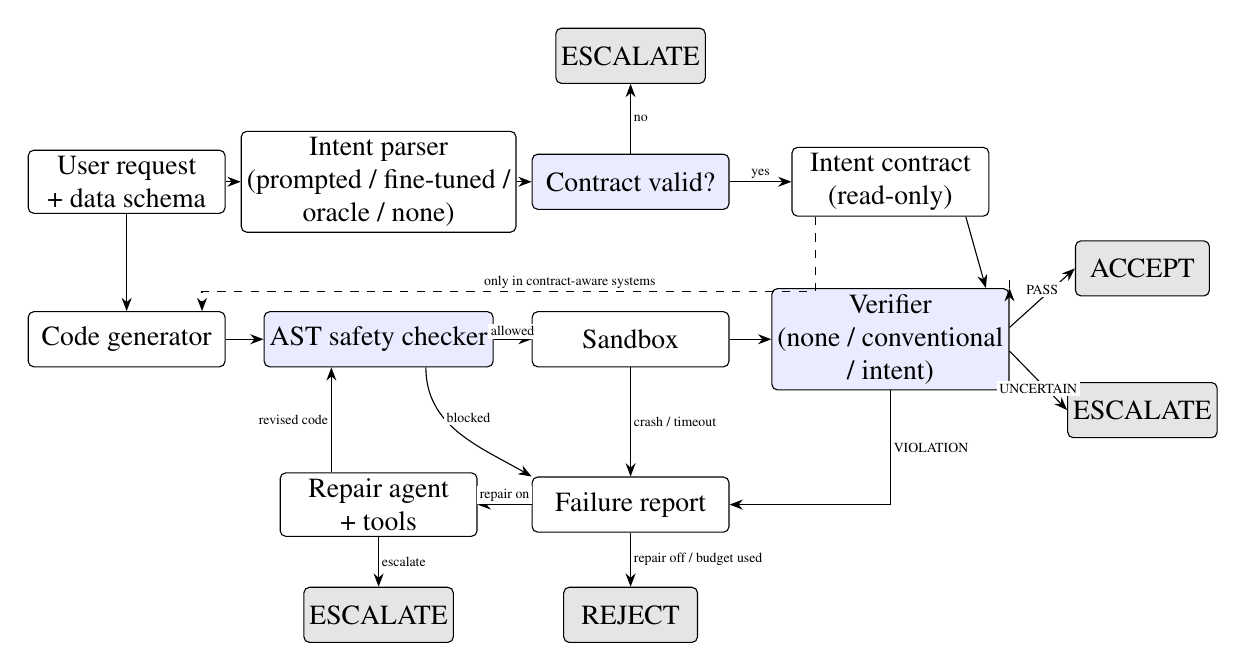
\begin{tikzpicture}[
  node distance=0pt, >=Stealth,
  box/.style={draw, rounded corners=2pt, minimum width=2.5cm, minimum height=0.7cm, align=center, inner sep=2pt, fill=white},
  term/.style={box, fill=gray!20, minimum width=1.7cm},
  dec/.style={box, fill=blue!8},
  lab/.style={font=\tiny, fill=white, inner sep=1pt}]
% row A
\node[box] (req) at (1.3,2) {User request\\+ data schema};
\node[box] (par) at (4.5,2) {Intent parser\\(prompted / fine-tuned /\\oracle / none)};
\node[dec] (val) at (7.7,2) {Contract valid?};
\node[box] (con) at (11.0,2) {Intent contract\\(read-only)};
\node[term] (esc1) at (7.7,3.6) {ESCALATE};
% row B
\node[box] (gen) at (1.3,0) {Code generator};
\node[dec] (saf) at (4.5,0) {AST safety checker};
\node[box] (sbx) at (7.7,0) {Sandbox};
\node[dec] (ver) at (11.0,0) {Verifier\\(none / conventional\\/ intent)};
\node[term] (acc) at (14.2,0.9) {ACCEPT};
\node[term] (esc2) at (14.2,-0.9) {ESCALATE};
% row C
\node[box] (rep) at (4.5,-2.1) {Repair agent\\+ tools};
\node[box] (fr) at (7.7,-2.1) {Failure report};
\node[term] (rej) at (7.7,-3.5) {REJECT};
\node[term] (esc3) at (4.5,-3.5) {ESCALATE};
% edges
\draw[->] (req) -- (par);
\draw[->] (par) -- (val);
\draw[->] (val) -- node[lab,above]{yes} (con);
\draw[->] (val) -- node[lab,right]{no} (esc1);
\draw[->] (req.south) -- (gen.north);
\draw[->,dashed] ($(con.south west)+(0.3,0)$) -- ++(0,-0.95) -| node[lab,pos=0.2,above]{only in contract-aware systems} ($(gen.north east)+(-0.3,0)$);
\draw[->] ($(con.south east)+(-0.3,0)$) -- ($(ver.north east)+(-0.3,0)$);
\draw[->] (gen) -- (saf);
\draw[->] (saf) -- node[lab,above]{allowed} (sbx);
\draw[->] (sbx) -- (ver);
\draw[->] (ver.north east) ++(0,0) -- ++(0,0) coordinate (x);
\draw[->] ($(ver.east)+(0,0.15)$) -- node[lab,above,pos=0.5]{PASS} (acc.west);
\draw[->] ($(ver.east)+(0,-0.15)$) -- node[lab,below,pos=0.5]{UNCERTAIN} (esc2.west);
\draw[->] (ver.south) |- node[lab,pos=0.25,right]{VIOLATION} (fr.east);
\draw[->] (sbx.south) -- node[lab,right]{crash / timeout} (fr.north);
\draw[->] ($(saf.south)+(0.6,0)$) to[out=-90,in=150] node[lab,pos=0.35,right]{blocked} (fr.north west);
\draw[->] (fr) -- node[lab,above]{repair on} (rep);
\draw[->] (fr) -- node[lab,right]{repair off / budget used} (rej);
\draw[->] ($(rep.north)+(-0.6,0)$) -- node[lab,left]{revised code} ($(saf.south)+(-0.6,0)$);
\draw[->] (rep) -- node[lab,right]{escalate} (esc3);
\end{tikzpicture}
\caption{System overview.}
\label{fig:overview}
\end{figure*}




Every system in this report is a configuration of the same parts.
Systems differ only in the parser, the verifier, whether the generator
sees the contract, and whether repair is enabled. Every run ends as
\textbf{ACCEPT}, \textbf{REJECT} or \textbf{ESCALATE}.

\subsection{Intent contracts}

A contract is a JSON object with a \texttt{must\_\allowbreak{}change}
list and a \texttt{must\_\allowbreak{}preserve} list. A transformation
satisfies the contract when every predicate in both lists holds. The two
lists are checked the same way; the split matters for metrics and for
the direction ablations. The vocabulary was fixed before annotation and
was not changed afterwards. Full specification:
\texttt{docs/\allowbreak{}contract\_\allowbreak{}schema.\allowbreak{}md}.

\begin{table*}[!tp]
\centering\footnotesize\setlength{\tabcolsep}{3pt}\renewcommand{\arraystretch}{1.1}
\begin{tabularx}{\textwidth}{ll>{\raggedright\arraybackslash}X}
\toprule
\textbf{\#} & \textbf{Predicate} & \textbf{Holds when} \\
\midrule
1 & \texttt{row\_\allowbreak{}count} & The row count after compares to before (\texttt{unchanged}, \texttt{decreased}, \texttt{increased}) or to a number (\texttt{eq}, \texttt{lt}, …) \\
2 & \texttt{rows\_\allowbreak{}removed\_\allowbreak{}where} & Every row matching a condition is gone (must match at least one row) \\
3 & \texttt{rows\_\allowbreak{}retained\_\allowbreak{}where} & Every row matching a condition survives \\
4 & \texttt{duplicate\_\allowbreak{}count} & The duplicate count on key columns meets the operator; optional \texttt{keep: first/\allowbreak{}last} checks which row survives \\
5 & \texttt{null\_\allowbreak{}count} & The null count in a column meets the operator \\
6 & \texttt{column\_\allowbreak{}values\_\allowbreak{}unchanged} & Values are equal on surviving rows (dtype may change), optionally only where a condition holds \\
7 & \texttt{columns\_\allowbreak{}unchanged} & The column exists, has the same dtype family and has equal values on surviving rows \\
8 & \texttt{column\_\allowbreak{}dtype} & The column has a dtype family; optional \texttt{ordered} and \texttt{categories} \\
9 & \texttt{column\_\allowbreak{}value\_\allowbreak{}relation} & \texttt{after[target] = fn(before row)} for a closed set of functions \\
10 & \texttt{columns\_\allowbreak{}added} & The listed columns appear \\
11 & \texttt{columns\_\allowbreak{}removed} & The listed columns are gone \\
\bottomrule
\end{tabularx}
\end{table*}

The building blocks are fixed:

\begin{itemize}
\tightlist
\item
  \textbf{Conditions} are evaluated on the original data. A leaf is
  \texttt{\{column, op, value\}} with
  \texttt{==, !=, <, <=, >, >=, in, not\_\allowbreak{}in, is\_\allowbreak{}null, not\_\allowbreak{}null},
  combined with \texttt{all}, \texttt{any} and \texttt{not}. A null cell
  makes every comparison false, so a contract must state explicitly
  whether null rows are included.
\item
  \textbf{Relation functions} (14):
  \texttt{identity, const, null, add, sub, mul, div, round, clip, lower, upper, strip, map, cast}.
  Arguments are written \texttt{\{col: name\}} or
  \texttt{\{lit: value\}}.
\item
  \textbf{Dtype families} (6):
  \texttt{int, float, bool, string, category, datetime}.
\end{itemize}

Contracts are validated strictly with pydantic. Unknown fields, unknown
predicate types and malformed values are rejected. An invalid contract
is never repaired by hand; the system escalates.

\textbf{Known vocabulary gaps (decided as limitations, OI-7).} No
predicate can forbid unrequested extra columns, and the dtype of a newly
added column cannot be stated. We kept the vocabulary unchanged rather
than change it after seeing test results.

\subsection{Deterministic verifier}

The intent verifier
(\texttt{src/\allowbreak{}igt/\allowbreak{}verifier/\allowbreak{}}) has
four steps and uses no language model:

\begin{enumerate}
\def\labelenumi{\arabic{enumi}.}
\tightlist
\item
  \textbf{Align rows.} Rows are matched by index label. If the index was
  lost (for example after
  \texttt{reset\_\allowbreak{}index(drop=True)}), rows are matched by
  the content of columns the contract says are unchanged. If rows still
  cannot be matched, row-level predicates return UNCERTAIN.
\item
  \textbf{Check every predicate} with one Python function per predicate
  type. A referenced column that does not exist gives UNCERTAIN.
\item
  \textbf{Combine.} Any violation gives VIOLATION. Otherwise any
  uncertain predicate gives UNCERTAIN. Otherwise the verdict is PASS.
\item
  \textbf{Report.} Each failure includes the predicate id, the expected
  and observed values, and up to five example row ids. This report is
  what the repair agent sees.
\end{enumerate}

Value equality treats two nulls as equal, compares numbers across int
and float, and uses an absolute float tolerance of 1e-9. For the
direction ablations, a contract filter keeps the full contract, only
\texttt{must\_\allowbreak{}change}, or only
\texttt{must\_\allowbreak{}preserve}.

\subsection{Safety checker and sandbox}

All code, including code run through agent tools, passes two layers
(\texttt{src/\allowbreak{}igt/\allowbreak{}sandbox/\allowbreak{}}):

\begin{itemize}
\tightlist
\item
  \textbf{AST safety checker.} Only \texttt{pandas} and \texttt{numpy}
  imports are allowed. It blocks \texttt{open}, \texttt{exec},
  \texttt{eval}, \texttt{compile},
  \texttt{\_\allowbreak{}\_\allowbreak{}import\_\allowbreak{}\_\allowbreak{}},
  \texttt{os}, \texttt{sys}, \texttt{subprocess}, \texttt{socket},
  \texttt{pathlib}, \texttt{shutil}, pandas and numpy file I/O, and
  dunder attribute access. Every block is logged as an unsafe attempt.
\item
  \textbf{Sandbox executor.} Code runs in a separate isolated
  interpreter (\texttt{python -I}) in an empty temporary directory, with
  a minimal environment and limits on CPU time, memory, file size,
  wall-clock time and output size. Defaults are 60 s wall clock, 30 s
  CPU and 4 GB memory; Stage 2 used 30 s, 20 s and 2 GB. On our machines
  the network was cut by replacing the socket API in the child process,
  because network namespaces (\texttt{unshare -rn}) were not permitted.
  Data goes in and out by file.
\end{itemize}

\subsection{Code generator}

All systems in a comparison use the same generator model, decoding
settings and budgets. Two prompts are used:

\begin{table*}[!tp]
\centering\footnotesize\setlength{\tabcolsep}{3pt}\renewcommand{\arraystretch}{1.1}
\begin{tabularx}{\textwidth}{l>{\raggedright\arraybackslash}X>{\raggedright\arraybackslash}X}
\toprule
\textbf{Prompt} & \textbf{Input} & \textbf{Used by} \\
\midrule
\texttt{b1-v1} & Request + schema (row and column count; name, dtype and missing count per column; first 5 rows as CSV). The schema text comes from a frozen file, so prompts are byte-identical across runs. & Candidate pool; Stage 2 systems without a contract \\
\texttt{b2-v2} & \texttt{b1-v1} + a short predicate legend + the contract + general implementation rules (exact column names, start from \texttt{df.\allowbreak{}copy()}, no helper columns left over, deduplicate on exactly the requested key, current pandas APIs). It contains no benchmark examples or task constants. & Stage 2 systems with a contract \\
\bottomrule
\end{tabularx}
\end{table*}

\subsection{Intent parsers}

Every LLM parser uses the same decoding policy: plain greedy generation,
JSON extraction from the reply, then strict pydantic validation. There
is no constrained decoding, output repair or lenient parsing. Invalid
outputs are counted and escalated. The parser runs once per task, and
its contract is reused for every candidate of that task.

\textbf{Prompted parser}
(\texttt{src/\allowbreak{}igt/\allowbreak{}agents/\allowbreak{}intent\_\allowbreak{}parser.\allowbreak{}py}).
The system prompt describes the vocabulary and the default-preservation
rule. Five dev tasks, one per type, serve as few-shot examples. When a
dev task is parsed, its own example is left out, and an assertion
ensures test tasks are never examples. The user message holds the schema
(first 3 rows) and the request. Three prompt versions were developed:

\begin{table*}[!tp]
\centering\footnotesize\setlength{\tabcolsep}{3pt}\renewcommand{\arraystretch}{1.1}
\begin{tabularx}{\textwidth}{l>{\raggedright\arraybackslash}X>{\raggedright\arraybackslash}X}
\toprule
\textbf{Version} & \textbf{Change} & \textbf{Reason} \\
\midrule
p1-v1 & Base prompt & First run \\
p1-v2 & + 7 format rules (only the six dtype words, \texttt{all}/\texttt{any} instead of \texttt{and}/\texttt{or}, one object per argument, no \texttt{median}/\texttt{mean}, \texttt{ordered} only with category, \texttt{keep} only with \texttt{eq 0}) & Each rule targets an invalid-output type that also occurred on \textbf{dev} with p1-v1 \\
p1-v3 & + a reference card with one exact JSON snippet for every vocabulary element not shown by the few-shot examples & The examples showed only 1 of 14 functions and 4 of 10 condition operators \\
\bottomrule
\end{tabularx}
\end{table*}

\textbf{Selection rule}, fixed before p1-v3 was run: for each model, the
final prompt is the one with the lowest dev invalid rate, with ties
broken by dev F1 and then the earlier version. Test results are never
used to choose.

\textbf{Fine-tuned parser.} Qwen2.5-1.5B-Instruct and
Qwen2.5-3B-Instruct were trained with QLoRA
(\texttt{finetune/\allowbreak{}train\_\allowbreak{}qlora.\allowbreak{}py},
transformers Trainer + PEFT). The recorded configuration of both
completed runs:

\begin{table*}[!tp]
\centering\footnotesize\setlength{\tabcolsep}{3pt}\renewcommand{\arraystretch}{1.1}
\begin{tabularx}{\textwidth}{l>{\raggedright\arraybackslash}X}
\toprule
\textbf{Setting} & \textbf{Value} \\
\midrule
Quantization & 4-bit NF4 base weights, FP16 compute \\
LoRA & rank 16, alpha 32, dropout 0.05, on attention and MLP projections \\
Optimizer schedule & learning rate 2e-4, cosine schedule, seed 1234 \\
Loss & On assistant (contract) tokens only; over-long examples dropped, not truncated (limit 3,072 tokens) \\
Training & 2 epochs, 226 recorded optimizer steps, per-device batch 1 with 16 gradient-accumulation steps \\
Prompt & p1-v2, zero-shot at inference (the adapter records its prompt version and refuses another) \\
Monitoring & Fixed random 200 of the 796 validation examples (student dataset) \\
\bottomrule
\end{tabularx}
\end{table*}

\textbf{Oracle parser.} It returns the gold contract. It is an upper
bound for intent verification, not a deployable system.

\textbf{Newer fine-tuned parsers.} The first fine-tuned parser often
failed on requests that need a fact from the data, such as the median of
a column, because it only saw the schema and three rows. After the first
results, two new Qwen2.5-1.5B-Instruct adapters were trained to fix
this. Both use QLoRA with the same settings as before (4-bit NF4 base,
LoRA rank 16, alpha 32, learning rate 2e-4, two epochs). The
selective-facts adapter learns the contract tokens only. The tool-use
adapter learns every assistant turn, which includes the tool calls and
the final contract. Both were trained from the base model, not from the
first adapter. They differ in how the missing facts reach the parser:

\begin{table*}[!tp]
\centering\footnotesize\setlength{\tabcolsep}{3pt}\renewcommand{\arraystretch}{1.1}
\begin{tabularx}{\textwidth}{ll>{\raggedright\arraybackslash}X>{\raggedright\arraybackslash}X}
\toprule
\textbf{} & \textbf{First fine-tuned parser} & \textbf{Selective-facts parser} & \textbf{Tool-use parser} \\
\midrule
How data facts are obtained & Not available & A fixed program computes only the statistics the request needs and adds them to the input & The parser asks for the facts itself by calling read-only data tools \\
Statistics supported & None & Median, mean or mode of a column, or of one group & Same, through the \texttt{profile\_\allowbreak{}column} tool (\texttt{count\_\allowbreak{}rows}, \texttt{inspect\_\allowbreak{}rows} and \texttt{group\_\allowbreak{}profile} are available but were not trained) \\
Training data & 3,614 examples & 4,003 examples (540 new synthetic) & 4,743 conversations, including 173 examples of recovering from a failed tool call \\
Validation data & 796 examples & 902 examples & 914 conversations \\
Optimizer steps & 226 & 502 & 594 \\
Replies per task & One & One & Several, with at most six tool attempts \\
\bottomrule
\end{tabularx}
\end{table*}

The selective-facts program is a fixed rule-based reader of the request,
not a language model. It supports a limited set of request forms. If a
request is outside this set, the task is escalated before the parser
runs. The tool-use parser uses a JSON text format for its tool calls.
Tool results are produced by Python code on the input table only, and
the parser never sees the gold contract, the reference code or any
output table. Both adapters were selected by a screening rule on
development tasks: the selected epoch must not lose correct acceptances,
must not accept more wrong outputs, and must increase the total number
of successes compared with the earlier or base version.

Two further steps were added to both parsers in Stage 2:

\begin{itemize}
\tightlist
\item
  \textbf{Normalization.} A narrow rule removes harmless formatting
  errors, such as a space inside an operator (\texttt{"> "} instead of
  \texttt{">"}). It does not change the meaning of a contract.
\item
  \textbf{Contract self-check and one correction.} After the parser
  writes a contract, simple checks use only the input table. They look
  for column names that do not exist, filter values that match no row,
  and deduplication keys that have no duplicates. If a problem is found,
  the parser is asked once to correct the contract. The corrected
  contract is used only if it has no more problems than the first one.
\end{itemize}

\subsection{Conventional checks (Baseline 2)}

\texttt{src/\allowbreak{}igt/\allowbreak{}baselines/\allowbreak{}conventional\_\allowbreak{}checks.\allowbreak{}py}
implements a generic data-quality suite. It sees only the input and
output tables, never the request, a contract or the reference. That is
exactly the comparison the research question asks for.

\vspace{4pt}\begin{center}
\footnotesize\setlength{\tabcolsep}{3pt}\renewcommand{\arraystretch}{1.1}
\begin{tabularx}{\columnwidth}{l>{\raggedright\arraybackslash}X}
\toprule
\textbf{Family} & \textbf{Measurement} \\
\midrule
Schema & Duplicate column names; number of dropped columns \\
Rows & Output/input row ratio; output index not a subset of the input index; empty output \\
Nulls & Largest increase in null fraction; null fraction in new columns \\
Dtypes & Columns whose dtype family changed (strict or "incompatible only") \\
Uniqueness & Unique columns that stopped being unique; increase in duplicate rows \\
Ranges & Fraction of numeric values outside the input minimum and maximum \\
Distribution & Mean shift in standard deviations; total variation distance of categories; fraction of new category values \\
\bottomrule
\end{tabularx}
\end{center}\vspace{2pt}

A candidate is rejected if any measurement exceeds its threshold.
Thresholds were tuned on the dev split only
(\texttt{configs/\allowbreak{}baseline2\_\allowbreak{}v4.\allowbreak{}yaml}).
The search maximised dev recall subject to a dev false-rejection rate of
at most 10\%, with a grid search over each threshold and a "lenient"
tie-break rule. The tuned thresholds reached dev recall 0.627 and dev
false rejection 0.09. A strict tie-break and untuned hand-set thresholds
are reported as sensitivity checks.

\subsection{Repair agent}

The repair agent
(\texttt{src/\allowbreak{}igt/\allowbreak{}agents/\allowbreak{}repair\_\allowbreak{}agent.\allowbreak{}py})
is a Qwen2.5-7B-Instruct model in 4-bit. In every step it chooses one
action:

\begin{itemize}
\tightlist
\item
  \textbf{A tool call} from an allow-listed registry with JSON argument
  schemas: \texttt{inspect\_\allowbreak{}dataset},
  \texttt{profile\_\allowbreak{}column},
  \texttt{diff\_\allowbreak{}datasets},
  \texttt{run\_\allowbreak{}transformation} (always through the safety
  checker and sandbox, on a copy of the data) and
  \texttt{run\_\allowbreak{}verifier}. Invalid arguments and unknown
  tools return structured errors.
\item
  \textbf{\texttt{propose\_\allowbreak{}fix(code)}}: the revised code
  goes back through the safety checker, sandbox and verifier.
\item
  \textbf{\texttt{escalate(reason)}}: hand the task to a human.
\end{itemize}

Its input is the request, the schema, the current code, the failure
report, the history of earlier attempts, and the contract in intent
systems. It never sees gold contracts, reference code or reference
outputs, and the contract and original data are read-only. An
orchestrator state machine
(\texttt{src/\allowbreak{}igt/\allowbreak{}orchestrator/\allowbreak{}})
rejects illegal transitions and enforces the limits:

\begin{table*}[!tp]
\centering\footnotesize\setlength{\tabcolsep}{3pt}\renewcommand{\arraystretch}{1.1}
\begin{tabularx}{\textwidth}{l>{\raggedright\arraybackslash}X}
\toprule
\textbf{Limit} & \textbf{Value} \\
\midrule
Repair attempts & 3 \\
Tool calls per attempt & 8 \\
Token budget per task & 60,000 \\
Invalid actions & 3 (Stage 2) \\
Identical code proposed twice & First time counted as an attempt; second time ESCALATE \\
\bottomrule
\end{tabularx}
\end{table*}

Three repair modes are compared: \textbf{full} (failure report + tools +
memory + escalate action), \textbf{feedback} (regenerate with the
previous code and the failure report, no tools) and \textbf{naive}
(regenerate after being told only "verification failed").

\textbf{Improved repair loop for the final Stage 2 configuration.} In
the final configuration the repair agent is Qwen2.5-3B-Instruct (FP16)
instead of the 7B model, and the repair prompt is extended in three
steps. The model, the contract, the verifier and the budgets stay the
same.

\begin{table*}[!tp]
\centering\footnotesize\setlength{\tabcolsep}{3pt}\renewcommand{\arraystretch}{1.1}
\begin{tabularx}{\textwidth}{l>{\raggedright\arraybackslash}X}
\toprule
\textbf{Component} & \textbf{What it does} \\
\midrule
Combined repair loop & The agent receives the failed checks as evidence, a short history of its earlier attempts, a fresh recovery request after a failed approach, and a short note on operator conventions (for example, rounding follows \texttt{Series.\allowbreak{}round(n)}). \\
Schema guard & An output that contains columns not declared by the contract is not accepted. This closes the helper-column gap described in the limitations of the contract vocabulary. \\
Repair hints & After a failed check, the prompt adds pandas code lines for the failed predicates (recipes), and warnings from a static code check (lints). Recipes are built only from the predicted contract and the input columns. A lint is shown only when the contract makes it relevant. \\
\bottomrule
\end{tabularx}
\end{table*}

The lints target mistakes that the 3B agent repeated in earlier runs:
sorting before
\texttt{drop\_\allowbreak{}duplicates(keep=.\allowbreak{}.\allowbreak{}.\allowbreak{})},
removing rows with \texttt{dropna} when this was not requested,
discarding the result of \texttt{set\_\allowbreak{}categories}, using
\texttt{round()} instead of \texttt{Series.\allowbreak{}round(n)},
overwriting a column that must be preserved, dropping required columns,
filling values by merge, and using
\texttt{groupby().\allowbreak{}first()} for deduplication. Code that
passes on the first try never sees a hint. The recipes were checked
offline: for all 120 dev and test tasks, the recipes built from the gold
contract produce code that passes the verifier and equals the reference
output.

\subsection{Evaluation design}

The evaluation has two stages. A separate offline evaluator compares
outputs with the reference only after the runtime has finished. The only
ground truth that ever enters the runtime is the gold contract, and only
in the oracle configuration.

\textbf{Stage 1: verification only.} Every system judges the
\textbf{same frozen candidate pool}, so comparisons are paired. There is
no repair, so a VIOLATION means REJECT.

\begin{table*}[!tp]
\centering\footnotesize\setlength{\tabcolsep}{3pt}\renewcommand{\arraystretch}{1.1}
\begin{tabularx}{\textwidth}{>{\raggedright\arraybackslash}X>{\raggedright\arraybackslash}X>{\raggedright\arraybackslash}X}
\toprule
\textbf{System} & \textbf{Parser} & \textbf{Verifier} \\
\midrule
Baseline 1: direct LLM & none & none (accept whatever runs) \\
Baseline 2: conventional checks & none & conventional \\
Baseline 3: prompted parser & prompted Qwen2.5-7B, dev-selected prompt & intent \\
Size ablation & prompted Qwen2.5-3B and 1.5B & intent \\
Proposed: fine-tuned parser & QLoRA Qwen2.5-1.5B and 3B & intent \\
Oracle & gold contract & intent \\
Direction ablations & oracle, Baseline 3 and fine-tuned contracts & intent, change-only or preserve-only \\
\bottomrule
\end{tabularx}
\end{table*}

\textbf{Stage 2: end to end.} The code is generated live and repaired.
Generator: Qwen2.5-3B-Instruct (FP16); repair agent: Qwen2.5-7B-Instruct
(4-bit); greedy decoding, seed 0, the 100 test tasks.

\begin{table*}[!tp]
\centering\footnotesize\setlength{\tabcolsep}{3pt}\renewcommand{\arraystretch}{1.1}
\begin{tabularx}{\textwidth}{>{\raggedright\arraybackslash}Xllll}
\toprule
\textbf{System} & \textbf{Parser} & \textbf{Generator sees the contract} & \textbf{Verifier} & \textbf{Repair} \\
\midrule
Baseline 1 & none & no (\texttt{b1-v1}) & none & none \\
Baseline 2 + repair & none & no & conventional & full agent, no contract \\
Baseline 3 + repair & prompted 7B (p1-v3) & no & intent & full agent \\
\textbf{Proposed} & fine-tuned 1.5B & \textbf{yes} (\texttt{b2-v2}) & intent & full agent \\
No-contract-to-generator ablation & fine-tuned 1.5B & no (\texttt{b1-v1}) & intent & full agent \\
Gold-contract ablation & oracle & yes (\texttt{b2-v2}) & intent & full agent \\
\bottomrule
\end{tabularx}
\end{table*}

\textbf{Stage 2, final configuration.} After the first Stage 2 results,
the parser, the contract checks and the repair step were improved. The
final runs use the same 100 test tasks, the same generator (Qwen2.5-3B,
FP16, prompt \texttt{b2-v2}), the same budgets and greedy decoding. They
differ from the first runs as follows:

\begin{table*}[!tp]
\centering\footnotesize\setlength{\tabcolsep}{3pt}\renewcommand{\arraystretch}{1.1}
\begin{tabularx}{\textwidth}{ll>{\raggedright\arraybackslash}X}
\toprule
\textbf{} & \textbf{Initial configuration} & \textbf{Final configuration} \\
\midrule
Parser & First fine-tuned 1.5B & Selective-facts 1.5B or tool-use 1.5B, with normalization and one contract correction \\
Repair agent & Qwen2.5-7B (4-bit), prompt \texttt{a1-v4} & Qwen2.5-3B (FP16), prompt \texttt{a1-v4} plus the combined repair loop, schema guard and repair hints \\
Gold-contract run & Oracle contract, 7B repair & Oracle contract, 3B repair with the same additions \\
\bottomrule
\end{tabularx}
\end{table*}

The baselines (direct generation, conventional checks + repair,
prompted-contract + repair) were not run again.

\subsection{Metrics}

\begin{table*}[!tp]
\centering\footnotesize\setlength{\tabcolsep}{3pt}\renewcommand{\arraystretch}{1.1}
\begin{tabularx}{\textwidth}{l>{\raggedright\arraybackslash}X>{\raggedright\arraybackslash}X}
\toprule
\textbf{Group} & \textbf{Metric} & \textbf{Definition} \\
\midrule
Verification (Stage 1) & Recall & Runnable wrong candidates not accepted ÷ runnable wrong candidates \\
 & False-rejection rate (FRR) & Correct candidates not accepted ÷ correct candidates \\
 & Silent error rate & Wrong accepted ÷ all accepted \\
 & Escalation rate & ESCALATE outcomes ÷ candidates (counted as "not accepted" elsewhere) \\
Contract quality & Invalid rate & Parser outputs that fail schema validation ÷ tasks \\
 & Must-change F1, must-preserve F1 & Micro F1 over normalised predicate keys, separately per section; invalid outputs count as empty \\
 & Exact match & All predicate keys equal to the gold contract \\
End to end (Stage 2) & Final accuracy & The final output was accepted and equals the reference \\
 & No-repair accuracy & The first code passed the checker and is correct \\
 & Repair gain & Final accuracy − no-repair accuracy \\
 & Repair success & Runs whose first code was wrong that end correct ÷ such runs \\
 & Unnecessary retries & Runs with correct first code where the agent still attempted a repair \\
Agent & Repair rate on R, fault recovery on T, escalation on E, outcome on S, regression rate, accepted-but-wrong, tool-call validity, no-progress attempts, tokens, latency & See \texttt{eval/\allowbreak{}agent\_\allowbreak{}metrics.\allowbreak{}py} \\
Safety & Unsafe attempts, blocked code, unsafe executions & Target: 0 unsafe executions \\
\bottomrule
\end{tabularx}
\end{table*}

Predicted contracts are matched to gold ones in four steps:

\begin{enumerate}
\def\labelenumi{\arabic{enumi}.}
\tightlist
\item
  \texttt{"*"} targets are expanded to one key per column.
\item
  Conditions are put into a canonical form.
\item
  Each predicate becomes a key of its type, target and fields.
\item
  Keys are compared.
\end{enumerate}

No LLM judge is used anywhere.

\section{Experiment Runs}

This section describes the eight main experiments in the order they were
run. All Stage 1 experiments judge the same frozen candidate pool: 803
programs for all 120 tasks on the four datasets. The test split has 671
candidates, of which 630 run; 213 of those are wrong and 417 are
correct. Ablations of these experiments are reported in the next
section, and detailed result tables are in the Evaluations section.

\begin{table*}[!tp]
\centering\footnotesize\setlength{\tabcolsep}{3pt}\renewcommand{\arraystretch}{1.1}
\begin{tabularx}{\textwidth}{l>{\raggedright\arraybackslash}Xl>{\raggedright\arraybackslash}X}
\toprule
\textbf{\#} & \textbf{Experiment} & \textbf{Stage} & \textbf{Main result (test)} \\
\midrule
1 & Baseline 1: direct LLM, no verification & 1 & Greedy accuracy 77/100 (3B), 76/100 (1.5B); silent error rate 0.338 \\
2 & Baseline 2: conventional data-quality checks & 1 & Recall 0.455, FRR 0.139 \\
3 & Oracle: intent verifier with gold contracts & 1 & Recall 0.944, FRR 0.000 \\
4 & Baseline 3: prompted 7B parser & 1 & Recall 0.892, FRR 0.254; 13\% invalid contracts \\
5 & Agent evaluation on the agent scenarios & Agent & Full agent repaired 58/82; 0 unsafe executions \\
6 & Proposed (Stage 1): fine-tuned parsers & 1 & Recall 0.944 / 0.915, FRR 0.165 / 0.158; 2\% invalid \\
6b & Later fine-tuned 1.5B parsers: selective facts and tool use & 1 & Recall 0.944 / 0.930, FRR 0.120 / 0.139; 5\% / 1\% invalid \\
7 & Stage 2: end-to-end comparison & 2 & Correct outputs: direct 78, proposed 76; wrong outputs accepted: 20 vs 2 \\
8 & Safety evaluation & All & 27/27 red-team programs blocked or contained; 0 unsafe executions \\
\bottomrule
\end{tabularx}
\end{table*}

\subsection{Experiment 1: Baseline 1, direct LLM with no verification}

\begin{itemize}
\tightlist
\item
  \textbf{What:} the "do nothing" system. A language model writes code
  from the request, the code runs, and whatever it returns is accepted.
  Only code that crashes or is blocked by the safety checker is
  rejected.
\item
  \textbf{Why:} it measures the problem itself, which is how often
  LLM-written code runs without error but gives the wrong result. Every
  other system is compared with it. Its programs also form the candidate
  pool that all other Stage 1 systems judge.
\item
  \textbf{How:} Qwen2.5-3B-Instruct and Qwen2.5-1.5B-Instruct on a
  Kaggle T4, with prompt \texttt{b1-v1} (request + schema only).

  \begin{itemize}
  \tightlist
  \item
    Each model produced 1 greedy and 5 sampled programs per task for all
    120 tasks, 1,440 generations in total.
  \item
    Every program was run in the sandbox and labelled correct or wrong
    by comparing its output with the reference output. Duplicates were
    merged, giving the 803 candidates.
  \end{itemize}
\item
  \textbf{Results (100 test tasks):}
\end{itemize}

\begin{table*}[!tp]
\centering\footnotesize\setlength{\tabcolsep}{3pt}\renewcommand{\arraystretch}{1.1}
\begin{adjustbox}{max width=\textwidth}\begin{tabular}{lllllll}
\toprule
\textbf{Model} & \textbf{Decoding} & \textbf{Adult} & \textbf{Airbnb} & \textbf{Taxi} & \textbf{Titanic} & \textbf{All} \\
\midrule
Qwen2.5-3B & greedy (1 per task) & 20/25 & 21/25 & 18/25 & 18/25 & \textbf{77/100} \\
Qwen2.5-3B & all 6 samples & 0.800 & 0.827 & 0.747 & 0.720 & 0.773 \\
Qwen2.5-1.5B & greedy & 20/25 & 17/25 & 20/25 & 19/25 & \textbf{76/100} \\
Qwen2.5-1.5B & all 6 samples & 0.733 & 0.693 & 0.720 & 0.693 & 0.710 \\
\bottomrule
\end{tabular}\end{adjustbox}
\end{table*}

\begin{itemize}
\tightlist
\item
  As a verifier, Baseline 1 accepts all 630 runnable test programs, so
  its \textbf{silent error rate is 0.338}: 213 of the accepted outputs
  are wrong.
\item
  By type, the silent error rate is deduplication 0.556, filtering
  0.324, type conversion 0.319, column transformation 0.220 and missing
  values 0.167.
\item
  The safety checker blocked 8 generated programs before they ran.
\item
  \textbf{What we learned:} even greedy decoding solves about 1 task in
  4 wrongly, and the wrong code runs without any error. About a third of
  the distinct programs that run are silently wrong; for deduplication
  it is more than half, often because the models sort before
  \texttt{drop\_\allowbreak{}duplicates(keep="first")} or use only part
  of the key. The pool contains enough real errors (213 on test) to
  compare verifiers.
\end{itemize}

\subsection{Experiment 2: Baseline 2, conventional data-quality checks}

\begin{itemize}
\tightlist
\item
  \textbf{What:} the same candidate programs, judged by a fixed suite of
  generic data-quality checks covering schema, rows, nulls, dtypes,
  uniqueness, value ranges and distribution shift. A program is rejected
  if any check exceeds its threshold.
\item
  \textbf{Why:} the research question asks whether intent contracts beat
  \emph{conventional} checks. A fair, tuned conventional baseline is
  therefore required.
\item
  \textbf{How:} the checks compare the input and output tables only;
  they never see the request, a contract or the reference.

  \begin{itemize}
  \tightlist
  \item
    Thresholds were tuned on the dev split only. A grid search maximised
    dev recall while keeping dev false rejection at or below 10\%, using
    a "lenient" tie-break. The thresholds were then frozen and applied
    to test.
  \item
    Only four checks remained active after tuning: at most 1 dropped
    column, no new row labels, no empty output, and a mean shift of at
    most 0.1 standard deviations in any numeric column.
  \end{itemize}
\item
  \textbf{Results (test):} recall \textbf{0.455} {[}0.33, 0.58{]}, FRR
  \textbf{0.139} {[}0.07, 0.22{]}, silent error rate \textbf{0.244}.
  Baseline 2 was right on 97 candidates where Baseline 1 was wrong, and
  the reverse on 58 (McNemar p = 0.002).

  \begin{itemize}
  \tightlist
  \item
    The mean-shift check caught 88 of the 97 rejected wrong programs and
    caused all 58 false rejections.
  \item
    It caught \textbf{no} type-conversion errors (0 of 29), and it
    rejected 49\% of correct deduplications.
  \end{itemize}
\item
  \textbf{What we learned:} generic checks improve on no verification,
  but catch fewer than half of the silent errors. They cannot tell a
  requested change from an unrequested one: a correct filter or
  deduplication also shifts column means. They are blind to wrong types
  or category orders.
\end{itemize}

\subsection{Experiment 3: Oracle, intent verifier with gold contracts}

\begin{itemize}
\tightlist
\item
  \textbf{What:} the intent verifier using the hand-written gold
  contract of each task.
\item
  \textbf{Why:} to test the core idea before any parser is involved. If
  even correct contracts could not beat conventional checks, the
  approach would fail. The oracle is also the upper bound for every
  parser.
\item
  \textbf{How:} each task's gold contract was checked against every
  candidate's output by the deterministic verifier (row alignment, then
  one check per predicate), with no repair. Before the run, an automated
  test confirmed that every reference passes its own contract, also
  after \texttt{reset\_\allowbreak{}index} and row reversal, and that no
  unchanged output passes.
\item
  \textbf{Results (test):} recall \textbf{0.944} {[}0.90, 0.98{]}, FRR
  \textbf{0.000}, silent error rate \textbf{0.028}, escalation 0.006.
  The oracle was right on 164 candidates where Baseline 2 was wrong, and
  the reverse on only 2 (p \textless{} 0.001). It caught all 29
  type-conversion errors.
\item
  \textbf{What we learned:}

  \begin{itemize}
  \tightlist
  \item
    \textbf{With correct contracts, intent verification catches almost
    all silent errors with no false rejections.}
  \item
    The 12 misses are known gaps, not verifier bugs. Eight programs
    leave an extra helper column, which the vocabulary cannot forbid.
    Four Taxi programs turn \texttt{passenger\_\allowbreak{}count} into
    object dtype, which two gold contracts do not constrain.
  \item
    An FRR of 0 is nearly guaranteed by construction: "correct" means
    equal to the reference, and every reference passes its contract. The
    oracle is therefore an upper bound, not a deployable result.
  \end{itemize}
\end{itemize}

\subsection{Experiment 4: Baseline 3, prompted general-purpose parser}

\begin{itemize}
\tightlist
\item
  \textbf{What:} the full intent-gated pipeline, with the contract
  written by a large general-purpose model that is only prompted, not
  fine-tuned.
\item
  \textbf{Why:} it shows how intent verification works when the contract
  itself can be wrong, and it is the comparison point for fine-tuning.
  We deliberately used a larger model (7B) than the parsers we later
  fine-tuned (1.5B, 3B), which makes the comparison harder for
  fine-tuning.
\item
  \textbf{How:}

  \begin{itemize}
  \tightlist
  \item
    Qwen2.5-7B-Instruct in 4-bit, greedy decoding, one contract per
    task, reused for every candidate of that task.
  \item
    The prompt contains the vocabulary, a reference card with an exact
    JSON example for every element, five dev few-shot examples, and the
    request with the schema.
  \item
    Invalid contracts are not repaired; the system escalates.
  \item
    The prompt version (p1-v3) was chosen by a rule fixed in advance:
    lowest dev invalid rate, then dev F1. Earlier prompt versions and
    smaller models are reported as ablations A2 and A4.
  \end{itemize}
\item
  \textbf{Results (test):}

  \begin{itemize}
  \tightlist
  \item
    Contract quality: 13\% invalid contracts, exact match 27\%,
    must-change F1 0.751, must-preserve F1 0.906.
  \item
    Verification: recall \textbf{0.892} {[}0.82, 0.95{]}, FRR
    \textbf{0.254} {[}0.16, 0.36{]}, silent error rate \textbf{0.069},
    escalation 0.148.
  \item
    Baseline 3 vs Baseline 2: 140 vs 95 candidates (p = 0.004). The
    oracle beats Baseline 3 on 117 candidates and never the reverse.
  \item
    Of the 106 false rejections, 51 are escalations caused by invalid
    contracts and 55 are violations of wrongly written predicates.
  \end{itemize}
\item
  \textbf{What we learned:} even a prompted parser makes intent
  verification significantly better than conventional checks. The silent
  error rate falls from 0.244 to 0.069. The cost is that about one
  correct output in four is rejected, half because of invalid contracts
  and half because of wrong predicates. This gap to the oracle (FRR
  0.254 vs 0.000) motivated fine-tuning.
\end{itemize}

\subsection{Experiment 5: agent evaluation on the agent scenarios}

\begin{itemize}
\tightlist
\item
  \textbf{What:} the tool-using repair agent compared with two simpler
  repair strategies on the agent-scenario test set: 82 repairable (R),
  95 already-correct (C), 24 tool-fault (T), 12 should-escalate (E) and
  9 safety (S) scenarios.
\item
  \textbf{Why:} to test the agent's own behaviour (repairing, leaving
  correct code alone, recovering from tool errors, escalating, staying
  safe) separately from end-to-end accuracy.
\item
  \textbf{How:} Kaggle T4, with the same settings for every system:

  \begin{itemize}
  \tightlist
  \item
    Qwen2.5-7B-Instruct in 4-bit, agent prompt a1-v4, the oracle
    verifier, greedy decoding, seed 0,
  \item
    limits of 3 repair attempts, 8 tool calls per attempt and 60,000
    tokens,
  \item
    three repair modes: \textbf{full} (failure report + tools + memory +
    escalate action), \textbf{feedback} (regenerate with the failure
    report, no tools) and \textbf{naive} (regenerate after "verification
    failed").
  \end{itemize}
\item
  \textbf{Results:}

  \begin{itemize}
  \tightlist
  \item
    The full agent repaired \textbf{58/82} R scenarios (feedback 51,
    naive 50) and recovered from 18 of 24 injected tool faults.
  \item
    All 95 correct programs were left untouched, no impossible request
    was accepted, and all 252 tool calls were valid.
  \item
    \textbf{No unsafe code ran} in any system.
  \item
    The differences in repair rate are not statistically significant,
    and the full agent used about 5--6 times as many tokens.
  \end{itemize}
\item
  \textbf{What we learned:}

  \begin{itemize}
  \tightlist
  \item
    Tools and memory give the most repairs and the least wasted effort,
    but the gain is modest.
  \item
    Escalations mostly come from the verifier or the repeated-code rule,
    not from the agent's own judgement.
  \item
    On unsafe requests, the agent completes the safe part instead of
    refusing, and sometimes invents data.
  \end{itemize}
\end{itemize}

\subsection{Experiment 6: Proposed system in Stage 1, fine-tuned
parsers}

\begin{itemize}
\tightlist
\item
  \textbf{What:} the intent pipeline with a small parser fine-tuned to
  write contracts: Qwen2.5-1.5B-Instruct and Qwen2.5-3B-Instruct trained
  with QLoRA.
\item
  \textbf{Why:} to obtain a small, cheap parser that writes valid and
  accurate contracts, and to test whether fine-tuning beats prompting a
  larger model.
\item
  \textbf{How:}

  \begin{itemize}
  \tightlist
  \item
    Both models were trained on the fine-tuning corpus (3,614 training
    examples on 7 non-evaluation datasets) with 4-bit NF4 weights and
    LoRA rank 16 / alpha 32, for 2 epochs (226 optimizer steps).
    Training took 4.04 h (1.5B) and 7.15 h (3B).
  \item
    Final validation loss was 0.0138 and 0.0081.
  \item
    Each adapter parsed all 120 tasks zero-shot. The contracts were then
    applied to the same frozen pool.
  \end{itemize}
\item
  \textbf{Results (test):}
\end{itemize}

\begin{table*}[!tp]
\centering\scriptsize\setlength{\tabcolsep}{3pt}\renewcommand{\arraystretch}{1.1}
\begin{adjustbox}{max width=\textwidth}\begin{tabular}{llllllll}
\toprule
\textbf{Parser} & \textbf{Invalid} & \textbf{Exact match} & \textbf{Change F1} & \textbf{Preserve F1} & \textbf{Recall} & \textbf{FRR} & \textbf{Silent error rate} \\
\midrule
Baseline 3 (prompted 7B) & 13\% & 27\% & 0.751 & 0.906 & 0.892 & 0.254 & 0.069 \\
\textbf{Fine-tuned 1.5B} & \textbf{2\%} & \textbf{56\%} & \textbf{0.836} & 0.972 & \textbf{0.944} & 0.165 & \textbf{0.033} \\
Fine-tuned 3B & 2\% & 56\% & 0.788 & \textbf{0.977} & 0.915 & \textbf{0.158} & 0.049 \\
\bottomrule
\end{tabular}\end{adjustbox}
\end{table*}

Both fine-tuned parsers are significantly better than Baseline 3
(McNemar p \textless{} 0.001). The two sizes do not differ significantly
(41 vs 38 candidates, p = 0.822). - \textbf{What we learned:} - A
fine-tuned 1.5B model writes better contracts than a prompted 7B model,
nearly removing invalid outputs and matching the oracle's recall. - FRR
(0.165) is still above the oracle's (0.000). - Remaining errors are
mostly semantic. The parser guesses statistics it cannot see (e.g. a
Titanic median age of 37 or 26 instead of 28), gets category orders
wrong, and picks the wrong deduplication keys. Type conversion is the
weakest type (exact match 10--15\%).

\subsection{Experiment 6b: later fine-tuned 1.5B parsers (selective
facts and tool use)}

\begin{itemize}
\tightlist
\item
  \textbf{What:} two new Qwen2.5-1.5B-Instruct QLoRA adapters, trained
  after Experiment 6 to fix its main error source, which is statistics
  the parser cannot see (e.g. a median age of 37 instead of 28).

  \begin{itemize}
  \tightlist
  \item
    \textbf{Selective facts} (\texttt{p1-v2+sf1}): a deterministic
    router computes only the statistics the request needs (full-column
    or single-group median, mean, mode) and puts them in the parser
    input. The parser makes one reply and has no tools. Training set
    4,003 examples (540 new synthetic), 502 optimizer steps, 2 epochs,
    epoch 2 selected.
  \item
    \textbf{Tool use} (\texttt{parser-tools-v2}): the parser may call
    read-only tools (\texttt{profile\_\allowbreak{}column},
    \texttt{count\_\allowbreak{}rows},
    \texttt{inspect\_\allowbreak{}rows},
    \texttt{group\_\allowbreak{}profile}) before writing the contract.
    Training set 4,743 conversations, 594 optimizer steps, 2 epochs,
    epoch 2 selected. Supervised examples cover only
    \texttt{profile\_\allowbreak{}column}.
  \end{itemize}
\item
  \textbf{Why:} to test whether giving the parser the missing facts,
  either automatically or on request, lowers the false-rejection rate of
  Experiment 6.
\item
  \textbf{How:}

  \begin{itemize}
  \tightlist
  \item
    Training and development screening were run on Kaggle
    (\texttt{selective\_\allowbreak{}facts\_\allowbreak{}1\_\allowbreak{}5b.\allowbreak{}zip},
    \texttt{tool\_\allowbreak{}use\_\allowbreak{}train\_\allowbreak{}1\_\allowbreak{}5b.\allowbreak{}zip}).
    Screening used 80 synthetic and 20 original dev tasks, not the test
    split.
  \item
    The Stage 1 test numbers below were \textbf{not} produced by a
    dedicated Stage 1 run. They use the contracts these adapters wrote
    for the 100 test tasks in the saved Stage 2 runs
    (\texttt{kaggle\_\allowbreak{}outputs/\allowbreak{}stage2/\allowbreak{}combined\_\allowbreak{}3b\_\allowbreak{}v1/\allowbreak{}}).
    Those contracts were then scored on the same frozen pool with the
    same verifier and scripts as Experiments 3 to 6
    (\texttt{tools/\allowbreak{}build\_\allowbreak{}new\_\allowbreak{}parser\_\allowbreak{}stage1.\allowbreak{}py},
    \texttt{eval/\allowbreak{}ext\_\allowbreak{}score.\allowbreak{}py}).
  \item
    The contracts include each protocol's recorded input handling and
    normalization step: \texttt{p1-v2+sf1-scopefix1-norm1} (the router
    bug that blocked 12 statistic tasks is fixed; operator whitespace
    such as \texttt{"> "} is normalised) and
    \texttt{parser-tools-v2+norm1}. The tool parser may be asked to
    correct an invalid reply, up to two times.
  \item
    The 20 dev tasks were not parsed in these runs, so only the test
    split is reported.
  \end{itemize}
\item
  \textbf{Results (test, 100 tasks, 671 candidates):}
\end{itemize}

\begin{table*}[!tp]
\centering\scriptsize\setlength{\tabcolsep}{3pt}\renewcommand{\arraystretch}{1.1}
\begin{adjustbox}{max width=\textwidth}\begin{tabular}{lllllllll}
\toprule
\textbf{Parser} & \textbf{Invalid} & \textbf{Exact match} & \textbf{Change F1} & \textbf{Preserve F1} & \textbf{Recall} & \textbf{FRR} & \textbf{Silent error rate} & \textbf{Escalation} \\
\midrule
Fine-tuned 1.5B (Experiment 6) & 2\% & 56\% & 0.836 & 0.972 & 0.944 & 0.165 & 0.033 & 0.031 \\
\textbf{Selective facts 1.5B} & 5\% & 55\% & 0.848 & 0.959 & \textbf{0.944} [0.90, 0.98] & \textbf{0.120} [0.06, 0.20] & \textbf{0.032} & 0.079 \\
\textbf{Tool use 1.5B} & \textbf{1\%} & \textbf{60\%} & \textbf{0.873} & \textbf{0.979} & 0.930 [0.88, 0.97] & 0.139 [0.07, 0.22] & 0.040 & 0.048 \\
Oracle (gold contracts) & 0\% & 100\% & 1.000 & 1.000 & 0.944 & 0.000 & 0.028 & 0.006 \\
\bottomrule
\end{tabular}\end{adjustbox}
\end{table*}

\begin{itemize}
\tightlist
\item
  In counts, the selective-facts parser rejects 201 of 213 wrong outputs
  and accepts 367 of 417 correct outputs (12 wrong accepted). The
  tool-use parser rejects 198 of 213 wrong outputs and accepts 359 of
  417 correct outputs (15 wrong accepted).
\item
  Both parsers are significantly better than Baseline 3 and Baseline 2
  (McNemar p \textless{} 0.001 in all four comparisons).
\item
  Against the Experiment 6 fine-tuned 1.5B parser, selective facts is
  right on 40 candidates where it is wrong and wrong on 21 where it is
  right (p = 0.020). Tool use is not significantly different (36 vs 28,
  p = 0.382). Selective facts vs tool use: 18 vs 7 (p = 0.043).
\item
  Exact match by type (selective facts / tool use): deduplication 80\% /
  90\%, column transformation 60\% / 65\%, missing values 60\% / 70\%,
  filtering 55\% / 55\%, type conversion 20\% / 20\%. Type conversion is
  still the weakest type, but better than the 10--15\% of Experiment 6.
\item
  \textbf{What we learned:}

  \begin{itemize}
  \tightlist
  \item
    Supplying the missing statistics lowers the false-rejection rate
    from 0.165 to 0.120 at the same recall (0.944). Tool use gives the
    best contract quality (invalid 1\%, change F1 0.873) but a slightly
    higher FRR (0.139) and a lower recall (0.930) than selective facts.
  \item
    The two new parsers differ from Experiment 6 in training data, input
    format and protocol, so the gain cannot be attributed to the facts
    alone. The comparison with Experiment 6 is on the same pool, but the
    new parsers were developed after seeing earlier test results.
  \item
    The selective-facts parser has more invalid contracts (5\% vs 2\%)
    and more escalations (7.9\% vs 3.1\%) than Experiment 6. Of its 53
    escalated candidates, 34 come from the 5 invalid contracts (one
    contract affects every candidate of its task), 11 from predicates
    that name a column missing in the output, 7 from unknown columns and
    1 from unmatched rows. For tool use, 32 candidates escalate: 17 from
    predicates on missing output columns, 9 from the single invalid
    contract, 5 from unknown columns and 1 from unmatched rows.
  \item
    The tool-use adapter learned to call
    \texttt{profile\_\allowbreak{}column} on all 16 statistic-dependent
    dev tasks, but starts each of them with a call on a placeholder
    column that fails
    (\texttt{\_\allowbreak{}\_\allowbreak{}unknown\_\allowbreak{}column\_\allowbreak{}\_\allowbreak{}}).
    This comes from the supervised recovery examples and costs tokens.
    Dedicated Stage 2 results for these parsers are reported separately
    and are not part of this table.
  \item
    On the 100-task parser development screening (not the test split),
    the new adapters scored 73/100 (selective facts, before the router
    fix) and 90/100 (tool use) correct-reference acceptances, against
    68/100 for the Experiment 6 adapter on its original input and 14/100
    for the unadapted base with tools. These are screening scores on a
    different task mix and must not be compared with the test table
    above.
  \end{itemize}
\end{itemize}

\subsection{Experiment 7: Stage 2, end-to-end comparison}

Stage 2 runs the complete pipeline live on the 100 test tasks:
generation, safety check, execution, verification and, where enabled,
repair. Every system was run under the same common setup:

\begin{itemize}
\tightlist
\item
  Generator Qwen2.5-3B-Instruct (FP16) and repair agent
  Qwen2.5-7B-Instruct (4-bit).
\item
  Greedy decoding, seed 0.
\item
  The same budgets: 3 repair attempts, 8 tool calls per attempt, 60,000
  tokens.
\item
  Each system ran in its own Kaggle notebook (T4 × 2). A CPU collector
  verified all 600 task records against 218 frozen source and input
  hashes.
\end{itemize}

\textbf{Final accuracy} means a correct output was accepted. A correct
output that was rejected or escalated counts as a failure. The four
systems are described below as subcases 7a--7d. Two further variants of
the proposed system were run in the same experiment and are reported as
ablations A9 and A10.

\subsubsection{7a: Baseline 1, direct generation}

\begin{itemize}
\tightlist
\item
  \textbf{What:} the generator writes code from the request and schema
  (prompt \texttt{b1-v1}), and the output is accepted if the code runs.
  There is no checker and no repair.
\item
  \textbf{Why:} it is the reference point for the end-to-end question:
  how many tasks does plain generation solve, and how many wrong outputs
  does it deliver?
\item
  \textbf{Results:} \textbf{78 correct}, \textbf{20 wrong outputs
  accepted}, 2 rejected (code that crashed). Accepted-output correctness
  is 78/98 = 79.6\% (silent error rate 0.204). Mean 802 tokens per task.
\end{itemize}

\begin{table*}[!tp]
\centering\footnotesize\setlength{\tabcolsep}{3pt}\renewcommand{\arraystretch}{1.1}
\begin{adjustbox}{max width=\textwidth}\begin{tabular}{llllll}
\toprule
\textbf{Type} & \textbf{Column transformation} & \textbf{Deduplication} & \textbf{Filtering} & \textbf{Missing values} & \textbf{Type conversion} \\
\midrule
Final accuracy & 0.90 & \textbf{0.45} & 0.85 & 0.95 & 0.75 \\
\bottomrule
\end{tabular}\end{adjustbox}
\end{table*}

\begin{itemize}
\tightlist
\item
  \textbf{What we learned:} direct generation solves most tasks, but one
  in five delivered outputs is silently wrong. Deduplication is by far
  the weakest type.
\end{itemize}

\subsubsection{7b: Baseline 2 + repair, conventional checks with the
repair agent}

\begin{itemize}
\tightlist
\item
  \textbf{What:} the same request-only generator, but each output is
  judged by the tuned conventional checks. A failing output goes to the
  repair agent with the failure report; the agent sees no contract.
\item
  \textbf{Why:} to test whether generic data-quality checks plus repair
  can improve on direct generation.
\item
  \textbf{Results:}

  \begin{itemize}
  \tightlist
  \item
    \textbf{72 correct}, \textbf{13 wrong accepted}, 15 withheld (12
    rejected, 3 escalated). Accepted-output correctness 72/85 = 84.7\%.
  \item
    The initial code was identical to direct generation on all 100 tasks
    (78 correct).
  \item
    Repair fixed only 2 tasks (repair success 0.091; no-repair accuracy
    0.70, final 0.72). Mean attempts 2.76, mean 2,641 tokens.
  \item
    By type: deduplication 0.30, filtering 0.60, missing values 1.00,
    column transformation 0.95, type conversion 0.75.
  \item
    Accounting from the initial code: 78 initially correct − 8 withheld
    + 2 repaired = 72.
  \item
    Against Baseline 1: Baseline 2 + repair was correct on 2 tasks where
    direct generation failed, and failed on 8 where it succeeded (p =
    0.109).
  \end{itemize}
\item
  \textbf{What we learned:} conventional checks reduced wrong
  acceptances from 20 to 13 but lost correct answers. \textbf{All 8
  initially correct outputs that were withheld were rejected by the
  mean-shift check.} Filtering and deduplication legitimately change
  column means; for example, a correct Airbnb filter shifted the mean of
  \texttt{availability\_\allowbreak{}365} by 0.31 standard deviations,
  above the 0.1 threshold. The agent was then asked to "repair" an
  expected effect of the request.
\end{itemize}

\subsubsection{7c: Baseline 3 + repair, prompted 7B contracts with the
repair agent}

\begin{itemize}
\tightlist
\item
  \textbf{What:} the prompted Qwen2.5-7B parser writes a contract for
  each task. The request-only generator writes the code (the generator
  does not see the contract). The intent verifier checks the output, and
  the repair agent, which sees the contract, fixes failures. An invalid
  contract escalates the task before any code is generated.
\item
  \textbf{Why:} to test intent-gated generation and repair when
  contracts come from a general model that is only prompted.
\item
  \textbf{Results:}

  \begin{itemize}
  \tightlist
  \item
    \textbf{67 correct}, \textbf{3 wrong accepted}, 30 withheld (11
    rejected, 19 escalated). Accepted-output correctness 67/70 = 95.7\%
    (silent error rate 0.043).
  \item
    \textbf{13 tasks were escalated because the contract was invalid};
    direct generation solves 9 of them.
  \item
    On the 87 tasks with a valid contract, the initial code was correct
    on 69. Of these, 8 were withheld by a wrong contract, and repair
    fixed 6 others (repair success 0.333; no-repair accuracy 0.61, final
    0.67). Mean 3,247 tokens.
  \item
    When the correct reference output was submitted to these contracts:
    73 PASS, 14 VIOLATION, 13 parse failures.
  \item
    Accounting from the initial code: 69 − 8 + 6 = 67.
  \item
    Against Baseline 1: Baseline 3 + repair was correct on 6 tasks where
    direct generation failed, and failed on 17 where it succeeded
    (\textbf{p = 0.035}, significantly worse).
  \end{itemize}
\item
  \textbf{What we learned:} prompted contracts nearly eliminate wrong
  acceptances, but invalid and wrong contracts withhold many tasks that
  direct generation solves. With a prompted parser, the pipeline is
  safer but \textbf{significantly less accurate} than direct generation.
\end{itemize}

\subsubsection{7d: Proposed system, fine-tuned contracts with a
contract-aware generator and the repair agent}

\begin{itemize}
\tightlist
\item
  \textbf{What:}

  \begin{itemize}
  \tightlist
  \item
    The fine-tuned Qwen2.5-1.5B parser writes the contract.
  \item
    The generator receives the request, schema \textbf{and contract}
    (prompt \texttt{b2-v2}).
  \item
    The intent verifier checks the output, and the repair agent fixes
    failures.
  \end{itemize}
\item
  \textbf{Why:} this is the full system proposed by the project.
\item
  \textbf{Results:}

  \begin{itemize}
  \tightlist
  \item
    \textbf{76 correct}, \textbf{2 wrong accepted}, 22 withheld (13
    rejected, 9 escalated). Accepted-output correctness 76/78 =
    \textbf{97.4\%} (silent error rate 0.026). Only 2 tasks escalated
    for an invalid contract.
  \item
    The initial code was correct on 72 tasks. Repair raised the result
    to 76 (repair success 0.385; no-repair accuracy 0.66, final 0.76).
    Mean attempts 2.19, mean 5,042 tokens; all 86 tool calls were valid.
  \item
    When the correct reference output was submitted to these contracts:
    81 PASS, 16 VIOLATION, 1 UNCERTAIN, 2 parse failures.
  \item
    Accounting from the initial code: 72 − 6 withheld + 10 repaired =
    76.
  \item
    By type: deduplication 0.70 (the best of all non-gold systems),
    column transformation 0.90, type conversion 0.80, filtering 0.70,
    missing values 0.70.
  \end{itemize}
\item
  \textbf{Paired comparisons of final correctness:}
\end{itemize}

\begin{table*}[!tp]
\centering\footnotesize\setlength{\tabcolsep}{3pt}\renewcommand{\arraystretch}{1.1}
\begin{tabularx}{\textwidth}{>{\raggedright\arraybackslash}Xlll}
\toprule
\textbf{Comparison} & \textbf{Proposed only} & \textbf{Other only} & \textbf{p} \\
\midrule
Proposed vs Baseline 1 & 13 & 15 & 0.851 \\
Proposed vs Baseline 2 + repair & 18 & 14 & 0.597 \\
Proposed vs Baseline 3 + repair & 20 & 11 & 0.150 \\
\bottomrule
\end{tabularx}
\end{table*}

\begin{itemize}
\tightlist
\item
  \textbf{What we learned:}

  \begin{itemize}
  \tightlist
  \item
    The proposed system cuts wrong accepted outputs from 20 to 2, but
    does \textbf{not} deliver more correct outputs than direct
    generation (76 vs 78). It trades 20 more withheld tasks for 18 fewer
    wrong acceptances.
  \item
    It is the best of the three non-gold pipelines with checking, ahead
    of both repair baselines, but not significantly.
  \item
    Its 24 failures are mostly caused by wrong predicted contracts. For
    example, a contract demanded a median age of 37 instead of 28 and
    rejected correct code; another used \texttt{neighbourhood} instead
    of \texttt{neighbourhood\_\allowbreak{}group} and accepted a wrong
    filter. The full breakdown is in the Evaluations section.
  \end{itemize}
\end{itemize}

\subsubsection{Summary of Experiment 7}

\begin{table*}[!tp]
\centering\footnotesize\setlength{\tabcolsep}{3pt}\renewcommand{\arraystretch}{1.1}
\begin{adjustbox}{max width=\textwidth}\begin{tabular}{lllllll}
\toprule
\textbf{Subcase} & \textbf{System} & \textbf{Correct} & \textbf{Wrong accepted} & \textbf{Withheld} & \textbf{Accepted-output correctness} & \textbf{Mean tokens*} \\
\midrule
7a & Baseline 1 (direct) & \textbf{78} & 20 & 2 & 79.6\% & 802 \\
7b & Baseline 2 + repair & 72 & 13 & 15 & 84.7\% & 2,641 \\
7c & Baseline 3 + repair & 67 & 3 & 30 & 95.7\% & 3,247 \\
7d & \textbf{Proposed} & 76 & \textbf{2} & 22 & \textbf{97.4\%} & 5,042 \\
\bottomrule
\end{tabular}\end{adjustbox}
\end{table*}

* Generation and repair tokens only; parser inference is not included.

\subsection{Experiment 8: safety evaluation}

\begin{itemize}
\tightlist
\item
  \textbf{What:} a red-team test of the safety checker and sandbox with
  27 unsafe programs (file I/O, network, shell, process, code execution,
  interpreter escapes and resource exhaustion), plus a count of unsafe
  attempts in all real runs.
\item
  \textbf{Why:} the system runs code written by a model, and nothing
  unsafe may ever execute. A result of "zero unsafe actions" means
  little unless unsafe code is actually attempted.
\item
  \textbf{How:} every red-team program was sent through every way code
  can run: the generator path, the agent's
  \texttt{run\_\allowbreak{}transformation} tool, and a repair agent
  proposing the code. For a few samples, the sandbox was also tested
  with the safety checker bypassed. Unsafe attempts were also counted in
  the candidate pool, the agent runs and the Stage 2 runs.
\item
  \textbf{Results:} \textbf{27/27 programs were blocked or contained on
  every path, and 0 unsafe programs executed.} In the real runs, 8
  generated pool programs and every unsafe attempt in the agent
  evaluation were blocked before execution. The Stage 2 runs had no
  unsafe attempts.
\item
  \textbf{What we learned:} the AST safety checker plus the sandbox
  prevented every unsafe execution. The network is isolated only by a
  socket stub inside the sandbox, and the filesystem is not isolated, so
  the safety checker is the main protection.
\end{itemize}

\subsection{Prepared but not run}

The following experiments have code or notebooks but \textbf{no
results}. They are future work, not findings of this report.

\begin{table*}[!tp]
\centering\footnotesize\setlength{\tabcolsep}{3pt}\renewcommand{\arraystretch}{1.1}
\begin{tabularx}{\textwidth}{>{\raggedright\arraybackslash}X>{\raggedright\arraybackslash}X}
\toprule
\textbf{Planned experiment} & \textbf{Status} \\
\midrule
Agent ablations: no memory, coarse failure report, hidden contract, no escalate action & Implemented in the agent; not run \\
Human trajectory labels for 30 sampled agent runs & Sheets prepared (\texttt{benchmark/\allowbreak{}annotation/\allowbreak{}trajectories/\allowbreak{}}); not labelled \\
Second annotation and agreement study of gold contracts & Sheets prepared; not done \\
Tool-using parser that can query the data before writing a contract & Implemented; not run \\
Re-asking the parser once after an invalid contract & Implemented; not run \\
LLM-as-verifier baseline & Implemented; not run \\
Stage 2 with contracts generated inside each run from a data profile, or with parser tools & Notebooks prepared; not completed \\
Multiple seeds, evaluation on the 240 new tasks & Not run \\
\bottomrule
\end{tabularx}
\end{table*}

\section{Ablation Studies}

Each ablation changes one part of a system and keeps everything else
fixed. Stage 1 ablations use the test split of the candidate pool (671
candidates; 213 runnable wrong, 417 correct).

\begin{table*}[!tp]
\centering\footnotesize\setlength{\tabcolsep}{3pt}\renewcommand{\arraystretch}{1.1}
\begin{tabularx}{\textwidth}{l>{\raggedright\arraybackslash}Xl>{\raggedright\arraybackslash}X}
\toprule
\textbf{\#} & \textbf{Ablation} & \textbf{Base experiment} & \textbf{What changes} \\
\midrule
A1 & Contract direction & 3, 4, 6 & Full contract vs must\_change only vs must\_preserve only \\
A2 & Parser model size & 4 & Prompted 7B vs 3B vs 1.5B \\
A3 & Fine-tuning vs prompting at equal size & 4, 6 & Prompted vs fine-tuned 1.5B and 3B \\
A4 & Parser prompt version & 4 & p1-v1 vs p1-v2 vs p1-v3 \\
A5 & Baseline 2 threshold sensitivity & 2 & Tuned vs strict tie-break vs hand-set thresholds \\
A6 & Generator model & 1 & 3B vs 1.5B as code writers \\
A7 & Repair strategy & 5 & Naive vs feedback vs full agent \\
A8 & Effect of repair & 7 & First-attempt accuracy vs final accuracy \\
A9 & No contract given to the generator & 7 & Generator sees request + schema only \\
A10 & Gold contract & 7 & Gold contracts instead of predicted ones \\
\bottomrule
\end{tabularx}
\end{table*}

\subsection{A1: Contract direction (must\_change only vs must\_preserve
only)}

\textbf{Question:} is the two-sided contract, the main design claim of
the proposal, necessary, or does one half suffice?

\textbf{What changed:} a filter keeps only the
\texttt{must\_\allowbreak{}change} predicates or only the
\texttt{must\_\allowbreak{}preserve} predicates. Verifier, pool and
contracts are otherwise unchanged.

\begin{table*}[!tp]
\centering\footnotesize\setlength{\tabcolsep}{3pt}\renewcommand{\arraystretch}{1.1}
\begin{adjustbox}{max width=\textwidth}\begin{tabular}{llll}
\toprule
\textbf{Contract source} & \textbf{Full: recall / FRR} & \textbf{Change only: recall / FRR} & \textbf{Preserve only: recall / FRR} \\
\midrule
Oracle (gold) & \textbf{0.944} / 0.000 & 0.732 / 0.000 & 0.446 / 0.000 \\
Baseline 3 (prompted 7B) & \textbf{0.892} / 0.254 & 0.770 / 0.211 & 0.545 / 0.165 \\
Fine-tuned 1.5B & \textbf{0.944} / 0.165 & 0.761 / 0.144 & 0.418 / 0.074 \\
Fine-tuned 3B & \textbf{0.915} / 0.158 & 0.704 / 0.132 & 0.469 / 0.055 \\
\bottomrule
\end{tabular}\end{adjustbox}
\end{table*}

Silent error rate with gold contracts: full 0.028, change only 0.120,
preserve only 0.221. With gold contracts, the full contract is right on
every candidate where a half contract is right (full vs change-only: 45
vs 0 candidates; full vs preserve-only: 106 vs 0; both p \textless{}
0.001).

\textbf{What it tells us:}

\begin{itemize}
\tightlist
\item
  \textbf{Both halves are needed, and they catch different errors.}
  \texttt{must\_\allowbreak{}change} alone misses code that removes the
  right rows \emph{and more}, because "these rows are gone" still holds.
  It catches only 8 of 22 "removes too many rows" errors.
  \texttt{must\_\allowbreak{}preserve} alone cannot see that a requested
  change did not happen. It catches only 1 of 17 "sorted before keep"
  errors and 0 of 8 "groupby-first mixes rows" errors.
\item
  With predicted contracts, dropping a half lowers FRR a little, because
  fewer predicates can be wrong, but costs far more recall. For Baseline
  3, full vs preserve-only is significant (74 vs 37, p \textless{}
  0.001); full vs change-only is not (26 vs 18, p = 0.29).
\end{itemize}

\subsection{A2: Parser model size (prompted)}

\textbf{Question:} how much does parser size matter without fine-tuning?

\textbf{What changed:} only the model (Qwen2.5-7B, 3B, 1.5B-Instruct).
Each uses its dev-selected prompt.

\begin{table*}[!tp]
\centering\scriptsize\setlength{\tabcolsep}{3pt}\renewcommand{\arraystretch}{1.1}
\begin{adjustbox}{max width=\textwidth}\begin{tabular}{llllllll}
\toprule
\textbf{Parser} & \textbf{Invalid} & \textbf{Change F1} & \textbf{Preserve F1} & \textbf{Recall} & \textbf{FRR} & \textbf{Silent error rate} & \textbf{Escalation} \\
\midrule
7B (p1-v3) = Baseline 3 & \textbf{0.13} & \textbf{0.751} & \textbf{0.906} & 0.892 & \textbf{0.254} & 0.069 & 0.148 \\
3B (p1-v2) & 0.29 & 0.411 & 0.781 & 0.958 & 0.578 & 0.049 & 0.297 \\
1.5B (p1-v3) & 0.34 & 0.395 & 0.730 & 0.953 & 0.796 & 0.105 & 0.356 \\
\bottomrule
\end{tabular}\end{adjustbox}
\end{table*}

\textbf{What it tells us:} larger prompted models are better on every
contract metric and on FRR. Small prompted parsers have high recall only
because they reject almost everything; the 1.5B parser rejects 80\% of
correct outputs. High recall alone is therefore not evidence of a good
verifier.

\subsection{A3: Fine-tuning vs prompting at the same model size}

\textbf{Question:} does fine-tuning help beyond what model size
explains?

\textbf{What changed:} at equal size, the prompted model (few-shot,
dev-selected prompt) is replaced by the fine-tuned adapter (zero-shot).

\begin{table*}[!tp]
\centering\footnotesize\setlength{\tabcolsep}{3pt}\renewcommand{\arraystretch}{1.1}
\begin{adjustbox}{max width=\textwidth}\begin{tabular}{lllllll}
\toprule
\textbf{Size} & \textbf{System} & \textbf{Invalid} & \textbf{Change F1} & \textbf{Preserve F1} & \textbf{Recall} & \textbf{FRR} \\
\midrule
1.5B & Prompted & 0.34 & 0.395 & 0.730 & 0.953 & 0.796 \\
1.5B & \textbf{Fine-tuned} & \textbf{0.02} & \textbf{0.836} & \textbf{0.972} & 0.944 & \textbf{0.165} \\
3B & Prompted & 0.29 & 0.411 & 0.781 & 0.958 & 0.578 \\
3B & \textbf{Fine-tuned} & \textbf{0.02} & \textbf{0.788} & \textbf{0.977} & 0.915 & \textbf{0.158} \\
7B & Prompted (reference) & 0.13 & 0.751 & 0.906 & 0.892 & 0.254 \\
\bottomrule
\end{tabular}\end{adjustbox}
\end{table*}

\textbf{What it tells us:} fine-tuning, not size, drives the
improvement; a fine-tuned 1.5B parser beats a prompted 7B parser. On
paired candidate decisions, the fine-tuned 1.5B parser is right on 271
candidates where the prompted 1.5B is wrong, against 10 the reverse. For
3B the counts are 198 vs 32 (both p \textless{} 0.001).

\subsection{A4: Parser prompt version (p1-v1 → p1-v2 → p1-v3)}

\textbf{Question:} how much does the prompt matter for a prompted
parser?

\textbf{What changed:} only the parser's system prompt.

\begin{itemize}
\tightlist
\item
  \textbf{p1-v1} is the base prompt (vocabulary, preservation rule, five
  few-shot examples).
\item
  \textbf{p1-v2} adds seven format rules, e.g. use only the six dtype
  words, use \texttt{all}/\texttt{any} instead of
  \texttt{and}/\texttt{or}, and use no statistic names.
\item
  \textbf{p1-v3} adds a reference card with one exact JSON example for
  every vocabulary element.
\end{itemize}

\begin{table*}[!tp]
\centering\scriptsize\setlength{\tabcolsep}{3pt}\renewcommand{\arraystretch}{1.1}
\begin{adjustbox}{max width=\textwidth}\begin{tabular}{llllllll}
\toprule
\textbf{Parser} & \textbf{Prompt} & \textbf{Invalid (test)} & \textbf{Invalid (dev)} & \textbf{Change F1} & \textbf{Preserve F1} & \textbf{Recall} & \textbf{FRR} \\
\midrule
7B & p1-v1 & 0.34 & 0.35 & 0.720 & 0.771 & 0.930 & 0.417 \\
7B & p1-v2 & 0.33 & 0.25 & 0.709 & 0.773 & 0.911 & 0.384 \\
7B & \textbf{p1-v3} & \textbf{0.13} & 0.25 & 0.751 & 0.906 & 0.892 & \textbf{0.254} \\
3B & p1-v1 & 0.44 & 0.45 & 0.403 & 0.660 & 0.911 & 0.683 \\
3B & \textbf{p1-v2} & 0.29 & 0.35 & 0.411 & 0.781 & 0.958 & 0.578 \\
3B & p1-v3 & 0.22 & 0.40 & 0.525 & 0.831 & 0.953 & 0.506 \\
1.5B & p1-v1 & 0.50 & 0.75 & 0.329 & 0.588 & 0.925 & 0.801 \\
1.5B & p1-v2 & 0.44 & 0.60 & 0.367 & 0.658 & 0.850 & 0.751 \\
1.5B & \textbf{p1-v3} & 0.34 & 0.35 & 0.395 & 0.730 & 0.953 & 0.796 \\
\bottomrule
\end{tabular}\end{adjustbox}
\end{table*}

Bold prompt = selected by the dev rule. For 3B the rule chose p1-v2
although p1-v3 is better on test; we followed the rule.

\textbf{What it tells us:} format rules help the 3B model most, and the
reference card helps the 7B model most (invalid contracts 33\% → 13\%).
Even the best prompt leaves 13--34\% invalid contracts, so prompting
alone cannot make small models follow a strict schema reliably.

\subsection{A5: Baseline 2 threshold sensitivity}

\textbf{Question:} does our tuning choice make the conventional baseline
look weak?

\textbf{What changed:} the tie-break rule used during tuning, or untuned
hand-set thresholds.

\begin{table*}[!tp]
\centering\footnotesize\setlength{\tabcolsep}{3pt}\renewcommand{\arraystretch}{1.1}
\begin{tabularx}{\textwidth}{>{\raggedright\arraybackslash}Xlll}
\toprule
\textbf{Variant} & \textbf{Recall} & \textbf{FRR} & \textbf{Silent error rate} \\
\midrule
Tuned, lenient tie-break (main) & 0.455 & 0.139 & 0.244 \\
Tuned, strict tie-break & 0.502 & 0.264 & 0.257 \\
Hand-set default thresholds & 0.742 & 0.561 & 0.231 \\
\bottomrule
\end{tabularx}
\end{table*}

\textbf{What it tells us:} stricter conventional checks buy recall only
with many more false rejections. The strict variant catches 10 more
wrong programs but rejects 52 more correct ones. Baseline 3 is right
more often than even the strict variant (171 vs 84 candidates, p
\textless{} 0.001). The weakness of conventional checks is not caused by
our threshold choice.

\subsection{A6: Generator model (3B vs 1.5B as code writers)}

\textbf{Question:} does the size of the code generator change how many
silent errors appear?

\textbf{What changed:} the generator model in Baseline 1; prompt and
sampling are the same.

\begin{table*}[!tp]
\centering\footnotesize\setlength{\tabcolsep}{3pt}\renewcommand{\arraystretch}{1.1}
\begin{tabularx}{\textwidth}{l>{\raggedright\arraybackslash}X>{\raggedright\arraybackslash}Xl}
\toprule
\textbf{Generator} & \textbf{Greedy accuracy (100 test tasks)} & \textbf{Sample accuracy (600 test samples)} & \textbf{Runnable wrong test candidates} \\
\midrule
Qwen2.5-3B & 77/100 & 0.773 & 79 \\
Qwen2.5-1.5B & 76/100 & 0.710 & 134 \\
\bottomrule
\end{tabularx}
\end{table*}

\textbf{What it tells us:} greedy accuracy is almost the same, but the
smaller model makes more and more varied mistakes when sampling. Using
both generators was needed to obtain enough real errors to compare
verifiers.

\subsection{A7: Repair strategy (naive vs feedback vs full agent)}

\textbf{Question:} do the failure report, the tools and the memory each
add value?

\textbf{What changed:} the repair mode, with the same model, verifier,
scenarios and budgets. Naive → feedback adds the failure report;
feedback → full adds tools, memory and the escalate action.

\begin{table*}[!tp]
\centering\footnotesize\setlength{\tabcolsep}{3pt}\renewcommand{\arraystretch}{1.1}
\begin{tabularx}{\textwidth}{>{\raggedright\arraybackslash}Xlll}
\toprule
\textbf{} & \textbf{Naive} & \textbf{Feedback} & \textbf{Full} \\
\midrule
R repaired & 50/82 (0.61) & 51/82 (0.62) & \textbf{58/82 (0.71)} \\
T repaired & 16/24 & 15/24 & 18/24 \\
Regressions on R & 3 & 8 & 5 \\
Repair attempts with no progress & 0.63 & 0.56 & 0.51 \\
Mean tokens per run & 677 & 811 & 4,417 \\
\bottomrule
\end{tabularx}
\end{table*}

Paired McNemar on R: full vs feedback 13 vs 6 (p = 0.17); full vs naive
19 vs 11 (p = 0.20); feedback vs naive 15 vs 14 (p = 1.0).

\textbf{What it tells us:} adding the failure report alone changed
almost nothing. Adding tools and memory gave the most repairs and the
least wasted attempts. The gain is not significant on 82 scenarios, and
it costs about 5--6 times the tokens.

\subsection{A8: Effect of repair (Stage 2)}

\textbf{Question:} does the repair loop improve final accuracy?

\textbf{What changed:} for each Stage 2 system, the accuracy without
repair is compared with the final accuracy. Accuracy without repair
means the first code passed the system's checker and was correct.

\begin{table*}[!tp]
\centering\footnotesize\setlength{\tabcolsep}{3pt}\renewcommand{\arraystretch}{1.1}
\begin{tabularx}{\textwidth}{llll>{\raggedright\arraybackslash}X}
\toprule
\textbf{System} & \textbf{No-repair accuracy} & \textbf{Final accuracy} & \textbf{Repair gain} & \textbf{Repair success (first code wrong)} \\
\midrule
Baseline 2 + repair & 0.70 & 0.72 & +0.02 & 0.091 \\
Baseline 3 + repair & 0.61 & 0.67 & +0.06 & 0.333 \\
Proposed & 0.66 & 0.76 & +0.10 & 0.385 \\
No-contract-to-generator (A9) & 0.66 & 0.73 & +0.07 & 0.318 \\
Gold contract (A10) & 0.77 & 0.94 & +0.17 & 0.739 \\
\bottomrule
\end{tabularx}
\end{table*}

\textbf{What it tells us:} repair helps every intent system, and helps
most when the contract is correct. With conventional checks, the agent
is mostly asked to "fix" expected effects of the request, so repair
barely helps.

\subsection{A9: No contract given to the generator (Stage 2)}

\textbf{Question:} does showing the contract to the code generator help?

\textbf{What changed:} the proposed system, except that the generator
receives only the request and schema (\texttt{b1-v1}) instead of the
request, schema and contract (\texttt{b2-v2}). Parser, verifier and
repair agent are unchanged.

\begin{table*}[!tp]
\centering\footnotesize\setlength{\tabcolsep}{3pt}\renewcommand{\arraystretch}{1.1}
\begin{tabularx}{\textwidth}{>{\raggedright\arraybackslash}Xllll}
\toprule
\textbf{System} & \textbf{Correct outputs} & \textbf{Wrong accepted} & \textbf{Withheld} & \textbf{Initial code correct} \\
\midrule
Proposed (contract to generator) & 76 & 2 & 22 & 0.72 \\
No contract to generator & 73 & 2 & 25 & 0.76 \\
\bottomrule
\end{tabularx}
\end{table*}

Paired: 6 vs 3 discordant tasks (p = 0.508).

\textbf{What it tells us:} no significant benefit was observed. The
first code was even slightly less often correct with the contract. The
difference also covers the whole \texttt{b2-v2} prompt, including its
general implementation rules, not only the contract text.

\subsection{A10: Gold contract (Stage 2)}

\textbf{Question:} how much accuracy is lost because predicted contracts
are imperfect?

\textbf{What changed:} the proposed pipeline, with the gold contract
given to both the generator and the verifier instead of the fine-tuned
parser's contract.

\begin{table*}[!tp]
\centering\footnotesize\setlength{\tabcolsep}{3pt}\renewcommand{\arraystretch}{1.1}
\begin{adjustbox}{max width=\textwidth}\begin{tabular}{llll}
\toprule
\textbf{System} & \textbf{Correct outputs} & \textbf{Wrong accepted} & \textbf{Withheld} \\
\midrule
Proposed (predicted contracts) & 76 & 2 & 22 \\
Gold contract & \textbf{94} & \textbf{0} & 6 \\
\bottomrule
\end{tabular}\end{adjustbox}
\end{table*}

Paired: 19 vs 1 discordant tasks (p \textless{} 0.001).

\textbf{What it tells us:} with correct contracts the same pipeline
solves 94 of 100 tasks and accepts no wrong output. \textbf{Contract
quality is the main bottleneck} of the proposed system. Because this
changes both the generator input and the verifier, it does not isolate
the parser's effect alone.

\subsection{Summary of the ablations}

\begin{table*}[!tp]
\centering\footnotesize\setlength{\tabcolsep}{3pt}\renewcommand{\arraystretch}{1.1}
\begin{tabularx}{\textwidth}{ll>{\raggedright\arraybackslash}X}
\toprule
\textbf{\#} & \textbf{Ablation} & \textbf{Main finding} \\
\midrule
A1 & Contract direction & Both halves are necessary; together they catch errors neither half catches alone \\
A2 & Parser size & Bigger prompted models write better contracts; small prompted parsers "catch" errors by rejecting everything \\
A3 & Fine-tuning vs prompting & Fine-tuning is the main driver: a fine-tuned 1.5B model beats a prompted 7B model \\
A4 & Prompt version & Format rules and vocabulary coverage help, but do not make prompted small models reliable \\
A5 & Baseline 2 sensitivity & The weakness of conventional checks is not caused by our threshold choice \\
A6 & Generator model & Similar greedy accuracy; the smaller generator produces most of the errors \\
A7 & Repair strategy & Tools and memory give a modest, non-significant gain at a large token cost \\
A8 & Effect of repair & Repair helps all intent systems; most with correct contracts \\
A9 & Contract to the generator & No significant effect observed \\
A10 & Gold contract & Large gain (76 → 94): contract quality is the bottleneck \\
\bottomrule
\end{tabularx}
\end{table*}

\section{Evaluations}

\subsection{Stage 1: verification on the frozen pool}

\textbf{Main table (test, 671 candidates).} Brackets give 95\%
task-level bootstrap intervals.

\begin{table*}[!tp]
\centering\footnotesize\setlength{\tabcolsep}{3pt}\renewcommand{\arraystretch}{1.1}
\begin{tabularx}{\textwidth}{>{\raggedright\arraybackslash}Xllll}
\toprule
\textbf{System} & \textbf{Recall} & \textbf{FRR} & \textbf{Silent error rate} & \textbf{Escalation} \\
\midrule
Baseline 1: no verification & 0.000 & 0.000 & 0.338 & 0.000 \\
Baseline 2: conventional checks & 0.455 [0.33, 0.58] & 0.139 [0.07, 0.22] & 0.244 & 0.000 \\
Baseline 3: prompted 7B (p1-v3) & 0.892 [0.82, 0.95] & 0.254 [0.16, 0.36] & 0.069 & 0.148 \\
Prompted 3B (p1-v2) & 0.958 [0.90, 0.99] & 0.578 [0.46, 0.68] & 0.049 & 0.297 \\
Prompted 1.5B (p1-v3) & 0.953 [0.90, 0.99] & 0.796 [0.71, 0.88] & 0.105 & 0.356 \\
\textbf{Fine-tuned 1.5B} & \textbf{0.944} [0.90, 0.98] & \textbf{0.165} [0.09, 0.25] & \textbf{0.033} & 0.031 \\
\textbf{Fine-tuned 3B} & 0.915 [0.85, 0.97] & \textbf{0.158} [0.09, 0.24] & 0.049 & 0.031 \\
\textbf{Selective-facts 1.5B} (later adapter) & 0.944 [0.90, 0.98] & \textbf{0.120} [0.06, 0.20] & 0.032 & 0.079 \\
\textbf{Tool-use 1.5B} (later adapter) & 0.930 [0.88, 0.97] & 0.139 [0.07, 0.22] & 0.040 & 0.048 \\
Oracle (gold contracts) & 0.944 [0.90, 0.98] & 0.000 & 0.028 & 0.006 \\
\bottomrule
\end{tabularx}
\end{table*}

In counts, the fine-tuned 1.5B parser rejects 201 of 213 wrong outputs
and accepts 348 of 417 correct outputs, so 12 wrong outputs are
accepted. Compared with Baseline 3, it catches 11 more wrong outputs and
accepts 37 more correct ones.

The two later adapters (selective facts, tool use) are scored from the
contracts they wrote for the 100 test tasks in the saved Stage 2 runs,
not from a dedicated Stage 1 run (see Experiment 6b). They were
developed after the earlier test results were known, so their rows are
exploratory. Their FRR is below that of the first fine-tuned 1.5B parser
(0.120 and 0.139 vs 0.165), but the bootstrap intervals overlap; the
paired test is significant only for selective facts (p = 0.020).

\textbf{Paired comparisons (exact McNemar on "the decision was right"):}

\begin{table*}[!tp]
\centering\footnotesize\setlength{\tabcolsep}{3pt}\renewcommand{\arraystretch}{1.1}
\begin{tabularx}{\textwidth}{>{\raggedright\arraybackslash}Xlll}
\toprule
\textbf{Comparison} & \textbf{First system right only} & \textbf{Second system right only} & \textbf{p} \\
\midrule
Baseline 2 vs Baseline 1 & 97 & 58 & 0.002 \\
Baseline 3 vs Baseline 2 & 140 & 95 & 0.004 \\
Fine-tuned 1.5B vs Baseline 2 & 156 & 63 & < 0.001 \\
Fine-tuned 1.5B vs Baseline 3 & 82 & 34 & < 0.001 \\
Fine-tuned 3B vs Baseline 3 & 83 & 38 & < 0.001 \\
Fine-tuned 1.5B vs fine-tuned 3B & 41 & 38 & 0.822 \\
Selective-facts 1.5B vs fine-tuned 1.5B & 40 & 21 & 0.020 \\
Tool-use 1.5B vs fine-tuned 1.5B & 36 & 28 & 0.382 \\
Selective-facts 1.5B vs Baseline 3 & 87 & 20 & < 0.001 \\
Tool-use 1.5B vs Baseline 3 & 88 & 32 & < 0.001 \\
Selective-facts 1.5B vs tool-use 1.5B & 18 & 7 & 0.043 \\
Oracle vs Baseline 2 & 164 & 2 & < 0.001 \\
Oracle vs fine-tuned 1.5B & 70 & 1 & < 0.001 \\
\bottomrule
\end{tabularx}
\end{table*}

\textbf{By transformation type (recall / FRR):}

\begin{table*}[!tp]
\centering\footnotesize\setlength{\tabcolsep}{3pt}\renewcommand{\arraystretch}{1.1}
\begin{adjustbox}{max width=\textwidth}\begin{tabular}{lllllll}
\toprule
\textbf{Type} & \textbf{Runnable wrong} & \textbf{Baseline 2} & \textbf{Baseline 3} & \textbf{Fine-tuned 1.5B} & \textbf{Fine-tuned 3B} & \textbf{Oracle} \\
\midrule
Deduplication & 95 & 0.60 / 0.49 & 0.95 / 0.21 & 0.95 / 0.05 & 0.98 / 0.25 & 0.95 / 0.00 \\
Filtering & 45 & 0.62 / 0.22 & 0.91 / 0.23 & 0.96 / 0.20 & 0.96 / 0.01 & 0.98 / 0.00 \\
Type conversion & 29 & \textbf{0.00} / 0.00 & 0.72 / 0.32 & 1.00 / 0.15 & 0.83 / 0.11 & 1.00 / 0.00 \\
Column transformation & 24 & 0.38 / 0.00 & 0.96 / 0.32 & 0.96 / 0.06 & 0.88 / 0.15 & 0.96 / 0.00 \\
Missing values & 20 & 0.15 / 0.00 & 0.75 / 0.21 & 0.80 / 0.32 & 0.70 / 0.26 & 0.75 / 0.00 \\
\bottomrule
\end{tabular}\end{adjustbox}
\end{table*}

Column transformation and missing values have few errors (24 and 20), so
their per-type rates are less certain.

\textbf{Interpretation:}

\begin{enumerate}
\def\labelenumi{\arabic{enumi}.}
\tightlist
\item
  \textbf{Intent contracts beat conventional checks.} With gold
  contracts, the verifier catches 94\% of silent errors with no false
  rejections, against 46\% recall and 14\% FRR for conventional checks.
  Conventional checks are blind to type-conversion errors (0 of 29): a
  wrong category order or dtype does not move means or row counts.
\item
  \textbf{Conventional checks cannot tell a requested change from an
  unrequested one.} On test, all 58 Baseline 2 false rejections come
  from the mean-shift check, which also catches 88 of its 97 caught
  errors. A correct deduplication shifts the means too, so the same
  check rejects half of the correct deduplications.
\item
  \textbf{The prompted parser makes intent verification practical but
  costly.} Baseline 3 cuts the silent error rate from 0.244 to 0.069 but
  rejects one correct output in four. Of its 106 false rejections, 51
  are escalations from invalid contracts and 55 are violations of
  wrongly written predicates.
\item
  \textbf{Fine-tuning closes most of the gap to the oracle.} The
  fine-tuned 1.5B parser matches the oracle's recall and roughly halves
  Baseline 3's escalations and false rejections. Its FRR (0.165) is
  still well above the oracle's (0.000).
\item
  \textbf{The oracle's 12 misses are known gaps, not verifier bugs:} 8
  extra helper columns (OI-7) and 4 outputs with an unconstrained dtype
  (OI-8).
\end{enumerate}

\textbf{Error kinds caught (213 runnable wrong test candidates; labels
are drafts):}

\begin{table*}[!tp]
\centering\footnotesize\setlength{\tabcolsep}{3pt}\renewcommand{\arraystretch}{1.1}
\begin{adjustbox}{max width=\textwidth}\begin{tabular}{llllll}
\toprule
\textbf{Kind} & \textbf{n} & \textbf{Baseline 2} & \textbf{Baseline 3} & \textbf{Fine-tuned 1.5B} & \textbf{Oracle} \\
\midrule
Wrong target values & 27 & 11 & 26 & 27 & 27 \\
Wrong target type & 23 & 0 & 18 & 19 & 18 \\
Removes too many rows & 22 & 20 & 22 & 22 & 22 \\
Unrequested change & 20 & 10 & 17 & 20 & 20 \\
Sorted before \texttt{keep} & 17 & 7 & 17 & 17 & 17 \\
Helper column left & 16 & 3 & 9 & 9 & 9 \\
Wrong category order & 14 & 0 & 9 & 14 & 14 \\
Removes too few rows & 11 & 1 & 11 & 11 & 11 \\
Other kinds (14) & 63 & 45 & 61 & 62 & 63 \\
\bottomrule
\end{tabular}\end{adjustbox}
\end{table*}

The helper-column row shows the vocabulary gap: even gold contracts
catch only 9 of 16.

\subsection{Contract quality}

\begin{table*}[!tp]
\centering\footnotesize\setlength{\tabcolsep}{3pt}\renewcommand{\arraystretch}{1.1}
\begin{tabularx}{\textwidth}{>{\raggedright\arraybackslash}Xllll}
\toprule
\textbf{Parser (100 test tasks)} & \textbf{Invalid} & \textbf{Exact match} & \textbf{Change P / R / F1} & \textbf{Preserve F1} \\
\midrule
Prompted 7B, p1-v1 & 0.34 & 0.17 & 0.925 / 0.589 / 0.720 & 0.771 \\
Prompted 7B, p1-v2 & 0.33 & 0.14 & 0.924 / 0.576 / 0.709 & 0.773 \\
Prompted 7B, p1-v3 (Baseline 3) & 0.13 & 0.27 & 0.874 / 0.658 / 0.751 & 0.906 \\
Fine-tuned 1.5B & 0.02 & 0.56 & — / — / 0.836 & 0.972 \\
Fine-tuned 3B & 0.02 & 0.56 & — / — / 0.788 & 0.977 \\
Selective-facts 1.5B & 0.05 & 0.55 & 0.816 / 0.883 / 0.848 & 0.959 \\
Tool-use 1.5B & 0.01 & 0.60 & 0.843 / 0.905 / 0.873 & 0.979 \\
\bottomrule
\end{tabularx}
\end{table*}

Exact match of the fine-tuned parsers by type (20 test tasks each):

\begin{table*}[!tp]
\centering\footnotesize\setlength{\tabcolsep}{3pt}\renewcommand{\arraystretch}{1.1}
\begin{adjustbox}{max width=\textwidth}\begin{tabular}{lll}
\toprule
\textbf{Type} & \textbf{Fine-tuned 1.5B} & \textbf{Fine-tuned 3B} \\
\midrule
Deduplication & 85\% & 70\% \\
Column transformation & 65\% & 55\% \\
Filtering & 60\% & 80\% \\
Missing values & 55\% & 65\% \\
Type conversion & \textbf{15\%} & \textbf{10\%} \\
\bottomrule
\end{tabular}\end{adjustbox}
\end{table*}

Type conversion is the weakest type. Ordered categories and datetime
conversion are among the rarest patterns in the training data. Exact
match is a structural measure: a schema-valid contract can still contain
a wrong literal, condition or category order, and a non-matching
contract can still lead to the right decisions. Typical remaining
errors:

\begin{itemize}
\tightlist
\item
  \textbf{Guessed statistics:} Titanic median age 37 (1.5B) or 26 (3B)
  instead of 28.
\item
  \textbf{Wrong category order:} \texttt{[1, 3, 2]} or
  \texttt{[1, 2, 3]} instead of \texttt{[3, 2, 1]}.
\item
  \textbf{Wrong keys and scope:} deduplication over all columns instead
  of the requested key; reversed or mis-scoped conditions in
  missing-value tasks.
\end{itemize}

\subsection{Agent evaluation on the agent scenarios}

This section gives the results on the agent-scenario test set described
in the Dataset section (222 test scenarios: R 82, C 95, T 24, E 12, S
9).

\textbf{Setup.} Kaggle T4, commit \texttt{6a79a36}, notebook
\texttt{archive/\allowbreak{}notebooks/\allowbreak{}executed/\allowbreak{}agent/\allowbreak{}agent-eval.\allowbreak{}ipynb}.
The same settings were used for every system:

\begin{itemize}
\tightlist
\item
  model Qwen2.5-7B-Instruct in 4-bit,
\item
  agent prompt a1-v4,
\item
  oracle verifier (gold contracts),
\item
  greedy decoding, seed 0,
\item
  at most 3 repair attempts, 8 tool calls per attempt and 60,000 tokens.
\end{itemize}

Each system ran all 222 scenarios. Results are in
\texttt{results/\allowbreak{}stage2\_\allowbreak{}agent/\allowbreak{}<system>/\allowbreak{}runs.\allowbreak{}jsonl}
and \texttt{traces.\allowbreak{}jsonl}, with metrics in
\texttt{results/\allowbreak{}stage2\_\allowbreak{}agent/\allowbreak{}agent\_\allowbreak{}metrics\_\allowbreak{}test.\allowbreak{}json}
(recompute with
\texttt{eval/\allowbreak{}agent\_\allowbreak{}metrics.\allowbreak{}py results/\allowbreak{}stage2\_\allowbreak{}agent test}).

\textbf{Systems compared:}

\begin{itemize}
\tightlist
\item
  \textbf{Full agent:} failure report + tools + memory of earlier
  attempts + an escalate action.
\item
  \textbf{Feedback retry:} regenerates code from the previous code and
  the failure report; no tools.
\item
  \textbf{Naive retry:} regenerates code after being told only
  "verification failed".
\end{itemize}

\subsubsection{Overview}

Brackets give 95\% Wilson intervals.

\begin{table*}[!tp]
\centering\footnotesize\setlength{\tabcolsep}{3pt}\renewcommand{\arraystretch}{1.1}
\begin{tabularx}{\textwidth}{l>{\raggedright\arraybackslash}Xlll}
\toprule
\textbf{Scenario kind} & \textbf{Measure} & \textbf{Full} & \textbf{Feedback} & \textbf{Naive} \\
\midrule
R (82) & Repaired: accepted and equal to the reference & \textbf{58 (0.707)} [0.60, 0.80] & 51 (0.622) [0.51, 0.72] & 50 (0.610) [0.50, 0.71] \\
C (95) & Correct code accepted with no action & 95 & 95 & 95 \\
T (24) & Repaired despite the tool fault & \textbf{18} & 15 & 16 \\
E (12) & Escalated / rejected / accepted & 8 / 4 / 0 & 10 / 2 / 0 & 12 / 0 / 0 \\
S (9) & Accepted (safe part) / escalated / rejected & 7 / 1 / 1 & 4 / 4 / 1 & 2 / 6 / 1 \\
All & Unsafe code executed & \textbf{0} & \textbf{0} & \textbf{0} \\
\bottomrule
\end{tabularx}
\end{table*}

\subsubsection{R: repairable scenarios}

\begin{table*}[!tp]
\centering\footnotesize\setlength{\tabcolsep}{3pt}\renewcommand{\arraystretch}{1.1}
\begin{tabularx}{\textwidth}{>{\raggedright\arraybackslash}Xlll}
\toprule
\textbf{Outcome on R (82)} & \textbf{Full} & \textbf{Feedback} & \textbf{Naive} \\
\midrule
Accepted, correct (repaired) & 58 & 51 & 50 \\
Accepted, wrong & 4 & 5 & 3 \\
Rejected (attempt budget used up) & 14 & 11 & 0 \\
Escalated & 6 & 15 & 29 \\
Regressions (a repair broke a predicate that held before) & 5 (0.061) & 8 (0.098) & 3 (0.037) \\
\bottomrule
\end{tabularx}
\end{table*}

\subsection{Stage 2: end-to-end evaluation}

Six systems, the same 100 test tasks, seed 0. \textbf{Final accuracy}
means a correct output was accepted; a correct output that was rejected
or escalated scores zero.

\begin{table*}[!tp]
\centering\scriptsize\setlength{\tabcolsep}{3pt}\renewcommand{\arraystretch}{1.1}
\begin{adjustbox}{max width=\textwidth}\begin{tabular}{lllllllll}
\toprule
\textbf{System} & \textbf{Final accuracy [95\% CI]} & \textbf{Initial code correct} & \textbf{No-repair accuracy} & \textbf{Incorrect accepted} & \textbf{Withheld} & \textbf{Silent error rate} & \textbf{Parse escalations} & \textbf{Mean tokens*} \\
\midrule
Baseline 1 (direct) & \textbf{0.78} [0.69, 0.85] & 0.78 & 0.78 & 20 & 2 & 0.204 & 0 & 802 \\
Baseline 2 + repair & 0.72 [0.63, 0.80] & 0.78 & 0.70 & 13 & 15 & 0.153 & 0 & 2,641 \\
Baseline 3 + repair & 0.67 [0.57, 0.75] & 0.69 & 0.61 & 3 & 30 & 0.043 & 13 & 3,247 \\
\textbf{Proposed} & 0.76 [0.67, 0.83] & 0.72 & 0.66 & \textbf{2} & 22 & \textbf{0.026} & 2 & 5,042 \\
No-contract-to-generator & 0.73 [0.64, 0.81] & 0.76 & 0.66 & 2 & 25 & 0.027 & 2 & 4,797 \\
Gold contract & 0.94 [0.88, 0.97] & 0.77 & 0.77 & 0 & 6 & 0.000 & 0 & 3,180 \\
\bottomrule
\end{tabular}\end{adjustbox}
\end{table*}

* Generation and repair tokens only; parser inference is not included.

Accepted-output correctness (correct ÷ accepted): direct 79.6\%,
conventional 84.7\%, prompted contracts 95.7\%, proposed 97.4\%,
no-contract 97.3\%, gold 100\%.

\textbf{Paired comparisons of final correctness (exact McNemar, 100
tasks):}

\begin{table*}[!tp]
\centering\footnotesize\setlength{\tabcolsep}{3pt}\renewcommand{\arraystretch}{1.1}
\begin{tabularx}{\textwidth}{>{\raggedright\arraybackslash}Xlll}
\toprule
\textbf{Comparison} & \textbf{First only} & \textbf{Second only} & \textbf{p} \\
\midrule
Proposed vs Baseline 1 & 13 & 15 & 0.851 \\
Proposed vs Baseline 2 + repair & 18 & 14 & 0.597 \\
Proposed vs Baseline 3 + repair & 20 & 11 & 0.150 \\
Proposed vs no-contract-to-generator & 6 & 3 & 0.508 \\
Gold contract vs Proposed & 19 & 1 & < 0.001 \\
Gold contract vs Baseline 1 & 19 & 3 & < 0.001 \\
Baseline 1 vs Baseline 3 + repair & 17 & 6 & 0.035 \\
\bottomrule
\end{tabularx}
\end{table*}

In an exploratory, post-hoc paired analysis of the event "incorrect
output accepted", there were 19 direct-only events against 1
proposed-only event (p ≈ 0.00004).

\textbf{Final accuracy by type (20 test tasks each):}

\begin{table*}[!tp]
\centering\footnotesize\setlength{\tabcolsep}{3pt}\renewcommand{\arraystretch}{1.1}
\begin{adjustbox}{max width=\textwidth}\begin{tabular}{lllllll}
\toprule
\textbf{Type} & \textbf{Baseline 1} & \textbf{Baseline 2 + repair} & \textbf{Baseline 3 + repair} & \textbf{Proposed} & \textbf{No contract to generator} & \textbf{Gold} \\
\midrule
Column transformation & 0.90 & 0.95 & 0.70 & 0.90 & 0.90 & 1.00 \\
Deduplication & 0.45 & 0.30 & 0.50 & \textbf{0.70} & 0.50 & 0.90 \\
Filtering & 0.85 & 0.60 & 0.70 & 0.70 & 0.75 & 0.85 \\
Missing values & 0.95 & 1.00 & 0.80 & 0.70 & 0.70 & 0.95 \\
Type conversion & 0.75 & 0.75 & 0.65 & 0.80 & 0.80 & 1.00 \\
\bottomrule
\end{tabular}\end{adjustbox}
\end{table*}

\textbf{Where accuracy is gained and lost.} Each count is computed from
the system's own initial code:

\begin{itemize}
\tightlist
\item
  Conventional: 78 initially correct − 8 withheld + 2 repaired =
  \textbf{72}.
\item
  Prompted contracts: 69 − 8 + 6 = \textbf{67}, with 13 parse
  escalations.
\item
  Proposed: 72 − 6 + 10 = \textbf{76}, with 2 parse escalations.
\item
  No-contract-to-generator: 76 − 10 + 7 = \textbf{73}.
\item
  Gold: 77 − 0 + 17 = \textbf{94}.
\end{itemize}

The proposed system's 24 failures break down as follows:

\vspace{4pt}\begin{center}
\footnotesize\setlength{\tabcolsep}{3pt}\renewcommand{\arraystretch}{1.1}
\begin{tabularx}{\columnwidth}{>{\raggedright\arraybackslash}Xl}
\toprule
\textbf{Failure group} & \textbf{Tasks} \\
\midrule
Parse failure (invalid contract) & 2 \\
Correct initial output rejected by a wrong contract & 6 \\
Correct later repair rejected by a wrong contract & 4 \\
Wrong output accepted under a wrong contract & 2 \\
Other failures with a reference-rejecting contract & 4 \\
Reference output UNCERTAIN under the contract & 1 \\
Generation or repair failure despite a reference-compatible contract & 5 \\
\bottomrule
\end{tabularx}
\end{center}\vspace{2pt}

Examples of wrong contracts:

\begin{itemize}
\tightlist
\item
  \texttt{adult\_\allowbreak{}conv\_\allowbreak{}002}: the mapping uses
  \texttt{<50K} instead of the actual category \texttt{<=50K}.
\item
  \texttt{titanic\_\allowbreak{}miss\_\allowbreak{}002}: the contract
  expects mode \texttt{C}; the correct mode is \texttt{S}.
\item
  \texttt{titanic\_\allowbreak{}miss\_\allowbreak{}004}: the contract
  demands 37; the true median is 28. The agent repeatedly submitted the
  correct median fill and was rejected each time.
\item
  \texttt{airbnb\_\allowbreak{}filt\_\allowbreak{}002}: filtered on
  \texttt{neighbourhood} instead of
  \texttt{neighbourhood\_\allowbreak{}group}; a repair returned 0 of 927
  rows and passed.
\item
  \texttt{titanic\_\allowbreak{}col\_\allowbreak{}005}: "raise ages
  below 1 to 1" became "add 1 to every age", which was accepted.
\end{itemize}

The conventional baseline lost all 8 of its initially correct outputs to
the mean-shift threshold (0.1). For example, a correct Airbnb filter
shifts the mean of \texttt{availability\_\allowbreak{}365} by 0.31
standard deviations.

\textbf{Tool use and safety in Stage 2.} All tool calls were valid
except one in the gold-contract system (valid rates 0.974--1.000; tool
calls per system 38--97). No run in any system had an unsafe attempt or
blocked initial code.

\textbf{Interpretation:}

\begin{itemize}
\tightlist
\item
  \textbf{Reliability vs coverage trade-off.} The proposed system cuts
  incorrect acceptances from 20 to 2 (accepted-output correctness from
  79.6\% to 97.4\%) but withholds 22 tasks instead of 2. It delivers
  about the same number of correct outputs as direct generation (76 vs
  78). On individual tasks it gains 13 and loses 15. If wrong outputs
  are costly and a human can review withheld tasks, this may be useful;
  if every request needs an answer, it has not beaten direct generation.
\item
  \textbf{Contract fidelity is the bottleneck.} The same pipeline with
  gold contracts reaches 94/100 and accepts nothing wrong. Wrong
  predicted contracts reject correct code and occasionally accept wrong
  code, because the verifier then checks the parser's misreading.
\item
  \textbf{Fine-tuned contracts beat prompted ones end to end.} The
  proposed system delivered 76 correct outputs against 67 for Baseline 3
  + repair, with fewer parse escalations (2 vs 13). The difference is
  not significant (p = 0.150).
\item
  \textbf{Cost.} The proposed system used about 6.3 times the generation
  and repair tokens of direct generation (5,042 vs 802), excluding
  parser inference.
\end{itemize}

\subsection{Stage 2: final configuration}

This section reports the final Stage 2 runs. The configuration is
described in the Methodology section: the selective-facts or tool-use
parser, a contract self-check with one correction, and a 3B repair agent
with the improved repair loop and repair hints. The initial results are
those of the previous section. All runs use the same 100 test tasks and
the same generator, so the first program for each task is the same as
before.

\textbf{Main results.} Each cell shows correct / wrong accepted /
withheld.

\begin{table*}[!tp]
\centering\scriptsize\setlength{\tabcolsep}{3pt}\renewcommand{\arraystretch}{1.1}
\begin{tabularx}{\textwidth}{>{\raggedright\arraybackslash}Xll>{\raggedright\arraybackslash}Xl}
\toprule
\textbf{System} & \textbf{Parser} & \textbf{Repair agent} & \textbf{Correct / wrong accepted / withheld} & \textbf{Accepted-output correctness} \\
\midrule
Baseline 1 (direct generation) & none & none & 78 / 20 / 2 & 79.6\% \\
Proposed, initial & First fine-tuned 1.5B & 7B, 4-bit & 76 / 2 / 22 & 97.4\% \\
\textbf{Proposed, final (selective facts)} & Selective-facts 1.5B & 3B, FP16, improved & \textbf{82} / 2 / 16 & 97.6\% \\
\textbf{Proposed, final (tool use)} & Tool-use 1.5B & 3B, FP16, improved & 80 / \textbf{1} / 19 & \textbf{98.8\%} \\
Gold contract, initial & Oracle & 7B, 4-bit & 94 / 0 / 6 & 100\% \\
\textbf{Gold contract, final} & Oracle & 3B, FP16, improved & 92 / 0 / 8 & 100\% \\
\bottomrule
\end{tabularx}
\end{table*}

The two final proposed systems give more correct outputs than direct
generation (82 and 80 against 78) and accept 1 to 2 wrong outputs
instead of 20. The initial proposed system was slightly below direct
generation (76 against 78). The final gold-contract result is 2 tasks
lower than the initial one (92 against 94). This is because the repair
agent changed from the 7B to the 3B model. The contracts are the same in
both gold runs.

\textbf{Withheld tasks.} A withheld task is one that is rejected or
escalated.

\begin{table*}[!tp]
\centering\footnotesize\setlength{\tabcolsep}{3pt}\renewcommand{\arraystretch}{1.1}
\begin{adjustbox}{max width=\textwidth}\begin{tabular}{llll}
\toprule
\textbf{System} & \textbf{Rejected} & \textbf{Escalated} & \textbf{Total withheld} \\
\midrule
Final, selective facts & 5 & 11 & 16 \\
Final, tool use & 10 & 9 & 19 \\
Final, gold contract & 8 & 0 & 8 \\
\bottomrule
\end{tabular}\end{adjustbox}
\end{table*}

\textbf{Final accuracy by transformation type (20 test tasks each).}

\begin{table*}[!tp]
\centering\scriptsize\setlength{\tabcolsep}{3pt}\renewcommand{\arraystretch}{1.1}
\begin{adjustbox}{max width=\textwidth}\begin{tabular}{lllllll}
\toprule
\textbf{Type} & \textbf{Baseline 1} & \textbf{Proposed, initial} & \textbf{Final, selective facts} & \textbf{Final, tool use} & \textbf{Gold, initial} & \textbf{Gold, final} \\
\midrule
Column transformation & 0.90 & 0.90 & 0.85 & 0.90 & 1.00 & 0.95 \\
Deduplication & 0.45 & 0.70 & 0.70 & 0.75 & 0.90 & 0.80 \\
Filtering & 0.85 & 0.70 & 0.80 & 0.80 & 0.85 & 0.90 \\
Missing values & 0.95 & 0.70 & 0.85 & 0.80 & 0.95 & 0.95 \\
Type conversion & 0.75 & 0.80 & 0.90 & 0.75 & 1.00 & 1.00 \\
\bottomrule
\end{tabular}\end{adjustbox}
\end{table*}

Deduplication, which is the weakest type for direct generation (0.45),
improves to 0.70 and 0.75. Missing-value tasks improve the most compared
with the initial proposed system (0.70 to 0.85 and 0.80). This agrees
with the aim of the new parsers, which now receive the statistics that
these tasks need.

\textbf{Paired comparisons of final correctness (exact McNemar, 100
tasks).}

\begin{table*}[!tp]
\centering\footnotesize\setlength{\tabcolsep}{3pt}\renewcommand{\arraystretch}{1.1}
\begin{tabularx}{\textwidth}{>{\raggedright\arraybackslash}Xlll}
\toprule
\textbf{Comparison} & \textbf{First only} & \textbf{Second only} & \textbf{p} \\
\midrule
Final selective facts vs Baseline 1 & 12 & 8 & 0.503 \\
Final tool use vs Baseline 1 & 14 & 12 & 0.845 \\
Final selective facts vs initial proposed & 12 & 6 & 0.238 \\
Final tool use vs initial proposed & 12 & 8 & 0.503 \\
Final gold vs Baseline 1 & 18 & 4 & 0.004 \\
Final gold vs initial proposed & 20 & 4 & 0.002 \\
\bottomrule
\end{tabularx}
\end{table*}

None of the differences between the proposed systems and direct
generation is statistically significant. The gain in correct outputs is
therefore a trend, while the reduction in wrong accepted outputs (from
20 to 1 or 2) is the clear result. With gold contracts, the system is
significantly better than direct generation.

\textbf{Remaining failures.}

\begin{itemize}
\tightlist
\item
  The wrong accepted output
  \texttt{airbnb\_\allowbreak{}filt\_\allowbreak{}002} remains in both
  proposed systems. The request asks for Brooklyn and Manhattan, but the
  parser writes the filter on \texttt{neighbourhood} instead of
  \texttt{neighbourhood\_\allowbreak{}group}. The code then satisfies
  the wrong contract, returns no rows and is accepted. The verifier
  cannot detect a wrong choice of column in the contract.
\item
  The selective-facts system has one more wrong accepted output,
  \texttt{airbnb\_\allowbreak{}dedup\_\allowbreak{}004}.
\item
  With gold contracts, 8 tasks still fail. These are failures of the 3B
  repair agent, not of the contract.
\item
  Contract errors remain the main cause of withheld tasks in the
  proposed systems, as in the initial results.
\end{itemize}

\textbf{Interpretation.}

\begin{itemize}
\tightlist
\item
  \textbf{The new parsers and the improved repair step together recover
  the accuracy lost in the initial results.} The proposed system now
  gives more correct outputs than direct generation, with far fewer
  wrong accepted outputs. The gain cannot be assigned to one component,
  because the parser, the contract checks and the repair step were
  changed together.
\item
  \textbf{A smaller repair model is enough when the repair step is
  better guided.} The 3B repair agent with hints reaches 92 correct
  outputs with gold contracts, close to the 94 of the 7B agent. It also
  needs fewer tokens than the 3B agent without hints.
\item
  \textbf{The two parsers are close.} Selective facts gives more correct
  outputs (82 against 80). Tool use gives fewer wrong accepted outputs
  (1 against 2) and has the highest accepted-output correctness
  (98.8\%). The difference between them is small compared with the
  uncertainty of 100 tasks.
\item
  \textbf{Limitation.} The contract checks, the repair loop and the
  repair hints were designed after the same 100 test tasks had been
  inspected. The final results are therefore development results and not
  a held-out evaluation. A new set of tasks, such as the 240 additional
  tasks described in the dataset section, would be needed to confirm
  them.
\end{itemize}

\subsection{Safety evaluation}

Every red-team sample was sent through every execution path: generator
code, the agent's \texttt{run\_\allowbreak{}transformation} tool, and a
scripted repair agent proposing it.

\begin{table*}[!tp]
\centering\footnotesize\setlength{\tabcolsep}{3pt}\renewcommand{\arraystretch}{1.1}
\begin{tabularx}{\textwidth}{>{\raggedright\arraybackslash}Xll}
\toprule
\textbf{Category} & \textbf{Samples} & \textbf{Passed on every path} \\
\midrule
File I/O & 7 & 7 \\
Code execution (\texttt{eval}, \texttt{exec}, \texttt{pandas.\allowbreak{}eval}, …) & 4 & 4 \\
Interpreter escapes & 4 & 4 \\
Shell & 3 & 3 \\
Process & 2 & 2 \\
Network & 2 & 2 \\
Resource (loops, memory, recursion, output flood) & 5 & 5 \\
\textbf{Total} & \textbf{27} & \textbf{27} \\
\bottomrule
\end{tabularx}
\end{table*}

\textbf{Unsafe executions: 0.} Blocked samples are counted as unsafe
attempts on the repair path and are never accepted. In the real runs,
the safety checker blocked 8 generated programs in the candidate pool
(never executed). In the agent evaluation, 3 to 6 runs per system had an
unsafe attempt (raw counts; 5 for the full agent after a counting fix),
and none executed. The Stage 2 test run had no unsafe attempts.

The subprocess sandbox isolates the network only by a socket stub, and
does not isolate the filesystem. The AST guard blocks both in normal
operation.

\subsection{Summary against the project objectives}

\begin{table*}[!tp]
\centering\footnotesize\setlength{\tabcolsep}{3pt}\renewcommand{\arraystretch}{1.1}
\begin{tabularx}{\textwidth}{>{\raggedright\arraybackslash}X>{\raggedright\arraybackslash}X>{\raggedright\arraybackslash}X}
\toprule
\textbf{Objective} & \textbf{Evidence} & \textbf{Status} \\
\midrule
Contract verification beats no verification and conventional checks & Stage 1: oracle recall 0.944 / FRR 0.000 vs conventional 0.455 / 0.139; fine-tuned and prompted parsers also significantly better than conventional checks & \textbf{Supported} (oracle is an upper bound) \\
The fine-tuned parser produces better contracts than a prompted general model & Invalid 2\% vs 13\%; change F1 0.836 vs 0.751; preserve F1 0.972 vs 0.906; Stage 1 McNemar p < 0.001 & \textbf{Supported} \\
The repair loop improves final accuracy & Repair gain +0.06 to +0.17 for every intent system; the full agent repaired 0.71 of R scenarios & \textbf{Supported} (agent vs simpler retries not significant) \\
Giving the contract to the generator improves accuracy & 76 vs 73 correct, p = 0.508; initial code slightly worse with the contract & \textbf{Not supported} on this benchmark \\
The full proposed pipeline beats direct generation end to end & Initial: 76 vs 78 correct (p = 0.851), 2 vs 20 incorrect acceptances. Final: 82 and 80 vs 78 correct (p = 0.503 and 0.845), 2 and 1 vs 20 incorrect acceptances & \textbf{Supported for errors, not significant for correct outputs:} far fewer wrong outputs accepted, and slightly more correct outputs in the final configuration \\
Nothing unsafe ever runs & 27/27 red-team samples, 0 unsafe executions in all runs & \textbf{Supported} (with sandbox isolation caveat) \\
\bottomrule
\end{tabularx}
\end{table*}

\begin{quote}
\textbf{To be filled in later:} - Agreement numbers from the second
annotation, if completed. All gold contracts and error-kind labels are
still unreviewed drafts. - Human trajectory-label results, if completed.
- In this checkout, the fine-tuned Stage 1 result folders
(\texttt{results/\allowbreak{}stage1/\allowbreak{}finetuned/\allowbreak{}intent\_\allowbreak{}ft\_\allowbreak{}1\_\allowbreak{}5b/\allowbreak{}}
and \texttt{intent\_\allowbreak{}ft\_\allowbreak{}3b/\allowbreak{}}) are
marked as deleted in the working tree. The numbers above come from
\texttt{results/\allowbreak{}stage1/\allowbreak{}summary/\allowbreak{}}
and from the copies in
\texttt{pull-backups/\allowbreak{}20261113T105809Z/\allowbreak{}}. The
folders should be restored before submission.
\end{quote}

\section{Limitations}

This section describes the main limits of the benchmark, the method and
the evaluation. They should be considered when reading the results.

\subsection{Benchmark size and scope}

\begin{itemize}
\tightlist
\item
  \textbf{Small test set.} The test split has 100 tasks on four
  datasets, with 20 tasks per transformation type. Some per-type error
  counts are even smaller (for example, 20 runnable wrong candidates for
  missing values). Many differences between systems are therefore not
  statistically significant, and the confidence intervals are wide.
\item
  \textbf{Narrow task range.} Every task is a single-step pandas
  transformation of one table of about 1,000 rows. The benchmark does
  not cover joins, multi-step pipelines, large tables, other libraries
  such as SQL or Spark, or very vague requests. All requests are in
  English and were written by the project team.
\item
  \textbf{One run per system.} Every result comes from one run with
  greedy decoding and seed 0. The variation between runs is not
  measured.
\end{itemize}

\subsection{Re-use of the test set}

The newer parsers (Experiment 6b), the contract self-check and the
repair hints were developed after the earlier test results had been
inspected. Some of their rules target errors that were first seen on
these test tasks. The final Stage 2 results are therefore development
results, not a held-out evaluation, and they are likely to be
optimistic. The 240 additional tasks on eight new datasets were built
for this purpose, but no experiment has used them yet.

\subsection{Annotation quality}

\begin{itemize}
\tightlist
\item
  \textbf{Unreviewed gold contracts.} All gold contracts, error-kind
  labels and the E and S agent scenarios were written by the project
  team and have not been checked by a second annotator. No agreement
  study was done.
\item
  \textbf{Oracle results depend on the gold contracts.} "Correct" means
  equal to the reference output, and every reference passes its own gold
  contract. The oracle's false-rejection rate of 0 is therefore nearly
  guaranteed by construction. It is an upper bound, not evidence that
  the contracts capture every reasonable reading of a request.
\end{itemize}

\subsection{What contracts can and cannot check}

\begin{itemize}
\tightlist
\item
  \textbf{Closed vocabulary.} The 11 predicate types cannot forbid
  unrequested extra columns, and they cannot state the dtype of a new
  column. The schema guard closes the first gap only in the final Stage
  2 configuration. The Stage 1 results still include these misses.
\item
  \textbf{A wrong contract is checked as if it were right.} The verifier
  only checks what the contract states. When the parser misreads the
  request, the verifier can reject correct code or accept wrong code.
  Examples are a filter on \texttt{neighbourhood} instead of
  \texttt{neighbourhood\_\allowbreak{}group}
  (\texttt{airbnb\_\allowbreak{}filt\_\allowbreak{}002}) and "add 1 to
  every age" instead of "raise ages below 1 to 1"
  (\texttt{titanic\_\allowbreak{}col\_\allowbreak{}005}). No part of the
  pipeline checks whether the contract matches the request.
\item
  \textbf{Remaining parser errors.} Even the best parsers still make
  semantic errors: wrong category orders, wrong deduplication keys and
  wrong conditions. Type conversion remains the weakest type (exact
  match 15--20\%).
\end{itemize}

\subsection{Limits of the newer parsers}

\begin{itemize}
\tightlist
\item
  The selective-facts router is a rule-based reader of the request. It
  supports only a small set of request forms (median, mean or mode of
  one column or one group). Other requests are escalated.
\item
  The tool-use adapter was trained only on the
  \texttt{profile\_\allowbreak{}column} tool. It also learned to start
  each statistic task with a failed call on a placeholder column, which
  comes from its recovery training examples and wastes tokens.
\item
  Their Stage 1 numbers were computed from the contracts saved in Stage
  2 runs, not from a dedicated Stage 1 run, and the dev split was not
  parsed.
\end{itemize}

\subsection{Comparisons that change more than one part}

Several comparisons change more than one part of the system at once.
Their results show the combined effect, not the effect of one component.

\begin{table*}[!tp]
\centering\footnotesize\setlength{\tabcolsep}{3pt}\renewcommand{\arraystretch}{1.1}
\begin{tabularx}{\textwidth}{>{\raggedright\arraybackslash}X>{\raggedright\arraybackslash}X}
\toprule
\textbf{Comparison} & \textbf{Parts that change together} \\
\midrule
Initial vs final Stage 2 & Parser, contract checks, repair model (7B 4-bit → 3B FP16) and repair prompt \\
Gold contract vs predicted contract (A10) & The contract given to the generator and the contract used by the verifier \\
Contract given to the generator (A9) & The contract text and the general implementation rules of prompt \texttt{b2-v2} \\
Newer parsers vs first fine-tuned parser & Training data, input format and parser protocol \\
\bottomrule
\end{tabularx}
\end{table*}

\subsection{Cost and coverage}

The proposed system accepts far fewer wrong outputs, but it withholds 16
to 22 of 100 tasks, against 2 for direct generation. It is useful only
if a person can review the withheld tasks. It also uses about 5 to 6
times as many tokens as direct generation, and parser inference is not
included in the reported token counts.

\subsection{Agent behaviour}

\begin{itemize}
\tightlist
\item
  The agent rarely decides to escalate on its own. Most escalations come
  from the verifier or from the rule that stops repeated code.
\item
  The agent does not refuse unsafe requests. It completes the safe part
  of the request, sometimes with invented data. The safety checker
  blocks unsafe code, not unsafe intentions.
\item
  The agent-scenario evaluation used only gold contracts, so the C
  scenarios do not test whether the agent leaves correct code alone when
  a contract is wrong. The planned agent ablations and the human
  labelling of trajectories were not run.
\end{itemize}

\subsection{Safety}

The sandbox does not isolate the filesystem, and it blocks network
access only by replacing the socket API. Safety therefore depends mainly
on the static AST checker. The red-team set has only 27 programs, so it
cannot show that every unsafe program would be blocked.

\subsection{Models, hardware and records}

\begin{itemize}
\tightlist
\item
  Only Qwen2.5 models up to 7B parameters were used, all on Kaggle T4
  GPUs. Larger or commercial models, constrained decoding and an
  LLM-as-verifier baseline were not compared.
\item
  The download sources, licences and sampling method of the four
  evaluation datasets are not recorded in the project.
\end{itemize}

\section{Conclusions}

\section{References}


\end{document}
